%============================================================
% BAB 3: LANDASAN TEORI
%   Flat list per teknologi/konsep, masing-masing jadi section.
%   Sub-section hanya untuk sub-fitur internal yang erat dengan induknya.
%============================================================
\chapter{LANDASAN TEORI}

Bab ini memuat teori-teori, konsep arsitektur, protokol komunikasi, basis data, kecerdasan buatan, dan teknologi rekayasa perangkat lunak yang menjadi landasan dalam pelaksanaan kerja praktik di \NamaPerusahaan. Seluruh bahasan disusun sebagai daftar datar (\textit{flat list}) per konsep maupun teknologi yang diterapkan pada tiga proyek kerja praktik, yaitu MonGrid, PT Makassar Trans, dan Nedo Agentic Platform.

%------------------------------------------------------------
\section{ARSITEKTUR \textit{MICROSERVICES}}
%------------------------------------------------------------

Arsitektur \textit{microservices} merupakan pendekatan perancangan perangkat lunak yang memecah sistem monolitik menjadi sekumpulan layanan kecil yang mandiri dan berfokus pada satu domain bisnis spesifik (\textit{bounded context})~\cite{newman2021building}. Setiap layanan menjalankan prosesnya sendiri, mengelola data atau tanggung jawabnya secara otonom, serta berkomunikasi melalui antarmuka jaringan terstandarisasi seperti HTTP/REST atau perantara pesan asinkron.

Keunggulan utama pendekatan ini meliputi isolasi kegagalan (\textit{fault isolation}) sehingga gangguan pada satu modul tidak langsung melumpuhkan keseluruhan sistem, kebebasan memilih teknologi (\textit{technology heterogeneity}) per layanan, serta kemampuan penskalaan horizontal dan pembaruan (\textit{deployment}) secara independen~\cite{newman2021building}. Meskipun demikian, arsitektur ini menuntut pengelolaan kompleksitas jaringan terdistribusi dan observabilitas yang lebih matang dibandingkan aplikasi monolitik tunggal. Perbandingan konseptual antara arsitektur monolitik dan \textit{microservices} diilustrasikan pada Gambar~\ref{fig:teori_microservices}.

\begin{figure}[H]
  \centering
  \IfFileExists{assets/gambar/landasan-teori/monolitik_vs_microservices.png}{%
    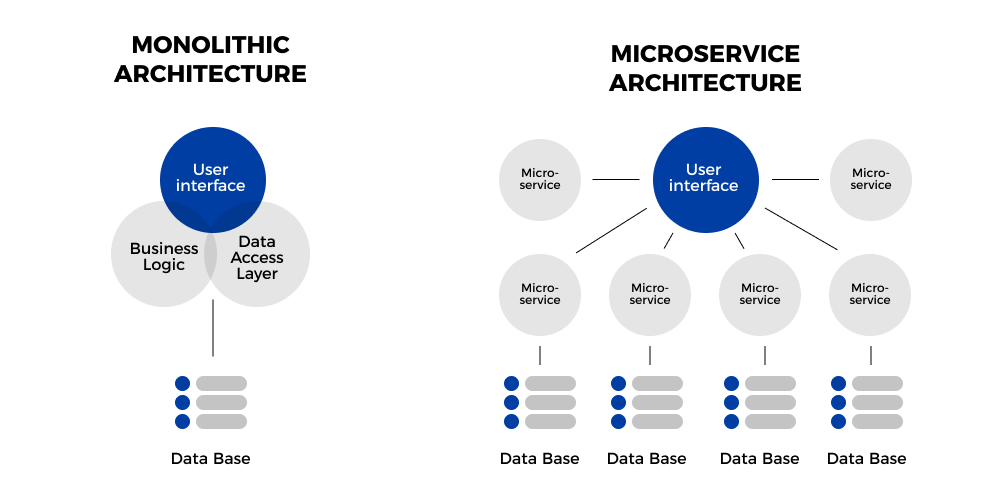
\includegraphics[width=0.9\textwidth,height=0.45\textheight,keepaspectratio]{assets/gambar/landasan-teori/monolitik_vs_microservices.png}%
  }{%
    \framebox[\textwidth][c]{\rule{0pt}{3.5cm}\parbox{0.82\textwidth}{\centering \textbf{[Placeholder Diagram: Perbandingan Arsitektur Monolitik dan \textit{Microservices}]}\\\textit{Menampilkan satu unit aplikasi dan basis data terpadu vs layanan-layanan independen terpisah. (Menunggu berkas gambar)}}}}
  \caption{Perbandingan Arsitektur Monolitik dan Arsitektur \textit{Microservices}}
  \label{fig:teori_microservices}
\end{figure}

Berdasarkan Gambar~\ref{fig:teori_microservices}, arsitektur monolitik mengemas seluruh logika bisnis ke dalam satu unit eksekusi dan satu skema basis data, sedangkan \textit{microservices} membagi sistem ke dalam layanan-layanan otonom yang dapat diskalakan secara terpisah. Pada proyek kerja praktik, MonGrid memisahkan layanan \textit{producer}, \textit{consumer}, layanan latar belakang, REST API, dan gerbang AI; PT Makassar Trans memisahkan aplikasi web operasional, worker OCR, dan layanan pengirim WhatsApp; sementara Nedo Agentic Platform memisahkan API Flask, pekerja Celery, \textit{Nedo LLM Gateway}, \textit{Runner Daemon}, serta layanan mikro MCP.

%------------------------------------------------------------
\section{ARSITEKTUR \textit{EVENT-DRIVEN}}
%------------------------------------------------------------

\textit{Event-Driven Architecture} (EDA) adalah paradigma perancangan sistem terdistribusi di mana komponen-komponen perangkat lunak berinteraksi melalui produksi, deteksi, dan konsumsi peristiwa (\textit{events}) yang merepresentasikan perubahan keadaan sistem secara asinkron~\cite{hohpe2003enterprise, newman2021building}. Alih-alih menunggu respons secara sinkron yang saling mengunci (\textit{blocking}), layanan pengirim cukup memancarkan peristiwa lalu melanjutkan eksekusinya.

Komponen inti dalam arsitektur ini terdiri atas \textit{Event Producer} (pembangkit peristiwa), \textit{Event Channel/Broker} (penyalur dan penyangga pesan), dan \textit{Event Consumer} (pemroses peristiwa)~\cite{hohpe2003enterprise}. Pemisahan ini menciptakan pelepasan ketergantungan waktu (\textit{temporal decoupling}) serta kemampuan menyerap lonjakan beban lalu lintas (\textit{burst buffering}) tanpa kehilangan data. Alur komunikasi dasar pada arsitektur berbasis peristiwa ditunjukkan pada Gambar~\ref{fig:teori_event_driven}.

\begin{figure}[H]
  \centering
  \IfFileExists{assets/gambar/landasan-teori/event_driven_architecture.png}{%
    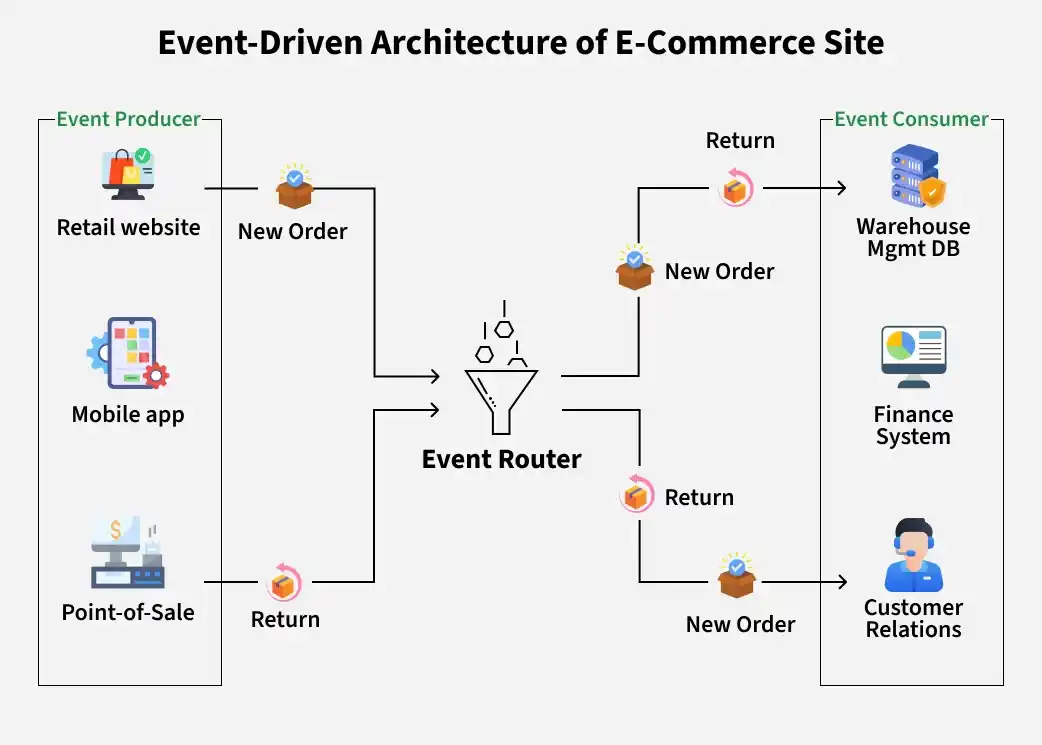
\includegraphics[width=0.9\textwidth,height=0.45\textheight,keepaspectratio]{assets/gambar/landasan-teori/event_driven_architecture.png}%
  }{%
    \framebox[\textwidth][c]{\rule{0pt}{3.5cm}\parbox{0.82\textwidth}{\centering \textbf{[Placeholder Diagram: Alur Komunikasi \textit{Event-Driven Architecture}]}\\\textit{Menampilkan alur Event Producer $\rightarrow$ Event Broker $\rightarrow$ Event Consumers secara asinkron. (Menunggu berkas gambar)}}}}
  \caption{Alur Komunikasi Dasar pada \textit{Event-Driven Architecture}}
  \label{fig:teori_event_driven}
\end{figure}

Sebagaimana diilustrasikan pada Gambar~\ref{fig:teori_event_driven}, peristiwa yang dihasilkan oleh produsen dialirkan melalui perantara pesan menuju satu atau lebih konsumen yang bereaksi secara mandiri. Pada proyek kerja praktik, paradigma ini diterapkan untuk mengalirkan telemetri sensor gardu dan peristiwa alarm di MonGrid serta memproses antrean verifikasi dokumen OCR dan pengiriman notifikasi WhatsApp di PT Makassar Trans.

%------------------------------------------------------------
\section{\textit{CLEAN ARCHITECTURE}}
%------------------------------------------------------------

\textit{Clean Architecture} yang diperkenalkan oleh Robert C. Martin adalah pola pengorganisasian kode perangkat lunak ke dalam lapisan-lapisan konsentris untuk menjaga agar logika bisnis inti tetap terisolasi dari detail teknis eksternal~\cite{martin2017clean}. Aturan fundamental dari arsitektur ini adalah \textit{The Dependency Rule}, yaitu ketergantungan kode sumber hanya diperbolehkan mengarah ke dalam menuju lapisan kebijakan yang lebih tinggi, dan lapisan dalam tidak boleh mengetahui rincian lapisan luar~\cite{martin2017clean}.

Struktur lapisan konsentris beserta arah ketergantungannya pada \textit{Clean Architecture} ditunjukkan pada Gambar~\ref{fig:teori_clean_arch}.

\begin{figure}[H]
  \centering
  \IfFileExists{assets/gambar/landasan-teori/clean_architecture.png}{%
    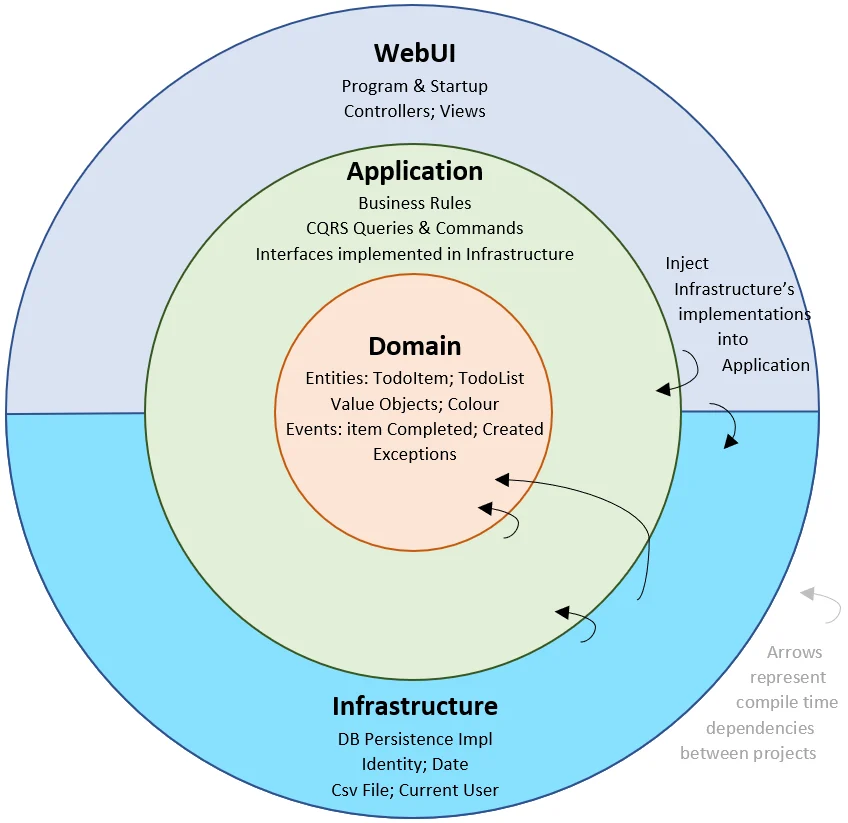
\includegraphics[width=0.85\textwidth,height=0.45\textheight,keepaspectratio]{assets/gambar/landasan-teori/clean_architecture.png}%
  }{%
    \framebox[\textwidth][c]{\rule{0pt}{3.5cm}\parbox{0.82\textwidth}{\centering \textbf{[Placeholder Diagram: Lapisan Konsentris \textit{Clean Architecture}]}\\\textit{Menampilkan lapisan Domain, Application, Infrastructure, dan API dengan arah Dependency Rule ke dalam. (Menunggu berkas gambar)}}}}
  \caption{Diagram Lapisan Konsentris dan \textit{Dependency Rule} pada \textit{Clean Architecture}}
  \label{fig:teori_clean_arch}
\end{figure}

Mengacu pada Gambar~\ref{fig:teori_clean_arch}, implementasi pola ini pada layanan \texttt{mongrid-backend} diwujudkan ke dalam empat lapisan tegas: \textit{Domain Layer} (entitas inti bebas dependensi), \textit{Application Layer} (antarmuka repositori, DTO, dan logika bisnis), \textit{Infrastructure Layer} (implementasi konkret akses PostgreSQL melalui Entity Framework Core, Redis, dan RabbitMQ), serta \textit{API Layer} (kontroler HTTP dan \textit{middleware}). Pemisahan ini memudahkan pengujian unit terhadap aturan bisnis tanpa ketergantungan pada infrastruktur basis data maupun jaringan nyata.

%------------------------------------------------------------
\section{\textit{REPRESENTATIONAL STATE TRANSFER} (REST) API}
%------------------------------------------------------------

\textbf{REST} (\textit{Representational State Transfer}) adalah gaya arsitektur perangkat lunak terdistribusi yang dirumuskan oleh Roy Fielding untuk sistem hipermedia berskala besar~\cite{fielding2000architectural}. Suatu layanan web dikategorikan mengikuti gaya REST apabila memenuhi enam batasan arsitektur utama, yakni pemisahan klien-server (\textit{client-server}), komunikasi nir-status (\textit{stateless}), dukungan tembolok (\textit{cacheable}), sistem berlapis (\textit{layered system}), antarmuka yang seragam (\textit{uniform interface}), serta opsi pengiriman kode sesuai permintaan (\textit{code on demand})~\cite{fielding2000architectural}.

Dalam praktik pengembangan antarmuka pemrograman aplikasi modern (\textit{RESTful JSON API}), setiap sumber daya diidentifikasi melalui alamat URI yang jelas dan dimanipulasi menggunakan metode HTTP standar, yaitu \texttt{GET} untuk membaca data, \texttt{POST} untuk membuat sumber daya baru, \texttt{PUT} atau \texttt{PATCH} untuk pembaruan, serta \texttt{DELETE} untuk penghapusan, disertai kode status HTTP yang semantik. Karena bersifat \textit{stateless}, setiap permintaan HTTP dari klien harus menyertakan seluruh konteks autentikasi dan parameter yang diperlukan tanpa bergantung pada memori sesi di server. Gaya arsitektur ini menjadi antarmuka komunikasi utama pada layanan web MonGrid (.NET 9), PT Makassar Trans (PHP), dan Nedo Agentic Platform (Flask).

%------------------------------------------------------------
\section{POLA KOMUNIKASI \textit{PUBLISH-SUBSCRIBE}}
%------------------------------------------------------------

\textit{Publish-Subscribe} (\textit{pub-sub}) adalah paradigma pertukaran pesan asinkron di mana pengirim (\textit{publisher}) mempublikasikan pesan ke sebuah saluran atau topik logis tanpa mengetahui identitas penerima, sedangkan penerima (\textit{subscriber}) mendaftarkan ketertarikannya pada topik tertentu untuk menerima salinan pesan secara otomatis~\cite{eugster2003many, rabbitmq_doc}. Dalam klasifikasinya, penyaringan pesan dapat berbasis topik (\textit{topic-based}) melalui pencocokan nama topik hierarkis maupun berbasis konten (\textit{content-based}) melalui evaluasi atribut pesan~\cite{eugster2003many}.

Keunggulan utama pola \textit{pub-sub} terletak pada pelepasan ikatan (\textit{decoupling}) dalam tiga dimensi sekaligus: \textit{space decoupling} (pengirim dan penerima tidak perlu saling mengetahui alamat jaringan), \textit{time decoupling} (keduanya tidak harus aktif pada waktu bersamaan bila ditopang perantara), dan \textit{synchronization decoupling} (aktivitas produksi dan konsumsi tidak saling memblokir)~\cite{eugster2003many}. Topologi komunikasi \textit{publish-subscribe} diperlihatkan pada Gambar~\ref{fig:teori_pubsub}.

\begin{figure}[H]
  \centering
  \IfFileExists{assets/gambar/landasan-teori/publish_subscribe.png}{%
    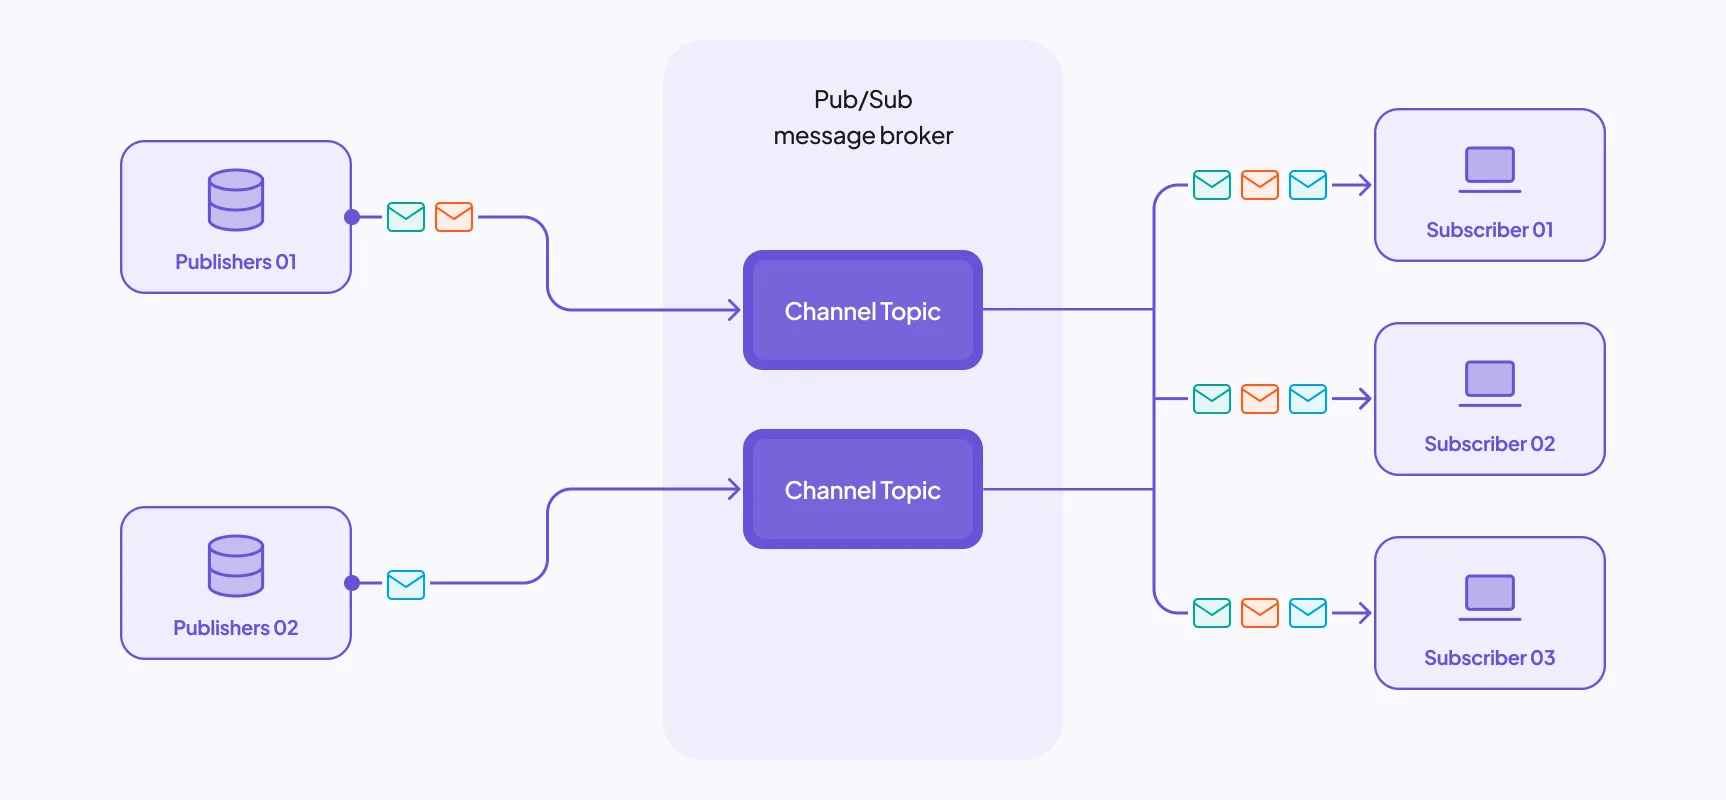
\includegraphics[width=0.9\textwidth,height=0.45\textheight,keepaspectratio]{assets/gambar/landasan-teori/publish_subscribe.png}%
  }{%
    \framebox[\textwidth][c]{\rule{0pt}{3.5cm}\parbox{0.82\textwidth}{\centering \textbf{[Placeholder Diagram: Topologi Pola Komunikasi \textit{Publish-Subscribe}]}\\\textit{Menampilkan Publishers mengirim ke Topic/Broker dan didistribusikan ke banyak Subscribers. (Menunggu berkas gambar)}}}}
  \caption{Topologi Pola Komunikasi \textit{Publish-Subscribe}}
  \label{fig:teori_pubsub}
\end{figure}

Berdasarkan Gambar~\ref{fig:teori_pubsub}, satu pesan yang dipublikasikan oleh produsen dapat disebarkan secara paralel ke banyak konsumen independen sesuai topik langganannya. Pola ini menjadi tulang punggung aliran telemetri sensor gardu pada MonGrid (melalui protokol MQTT) serta penyebaran pembaruan status perangkat dan sinyal kendali AI Chat (melalui RabbitMQ).

%------------------------------------------------------------
\section{PROTOKOL KOMUNIKASI AMQP}
%------------------------------------------------------------

\textbf{AMQP} (\textit{Advanced Message Queuing Protocol}), khususnya spesifikasi AMQP 0-9-1, adalah protokol lapis aplikasi berformat biner yang dirancang sebagai standar terbuka bagi \textit{message-oriented middleware}~\cite{amqp_spec, naik2017choice}. Berbeda dari protokol perpesanan sederhana yang hanya mengenal topik datar, AMQP mendefinisikan model perutean pesan yang dapat diprogram secara terperinci antara produsen dan konsumen, dengan dukungan multiplexing saluran (\textit{channels}) di atas satu koneksi TCP serta mekanisme konfirmasi penerimaan pesan (\textit{acknowledgement} / \texttt{basic.ack}) untuk menjamin keandalan pengiriman~\cite{amqp_spec}.

Model logis arsitektur pemetaan pesan pada protokol AMQP 0-9-1 diilustrasikan pada Gambar~\ref{fig:teori_amqp}.

\begin{figure}[H]
  \centering
  \IfFileExists{assets/gambar/landasan-teori/amqp_model.png}{%
    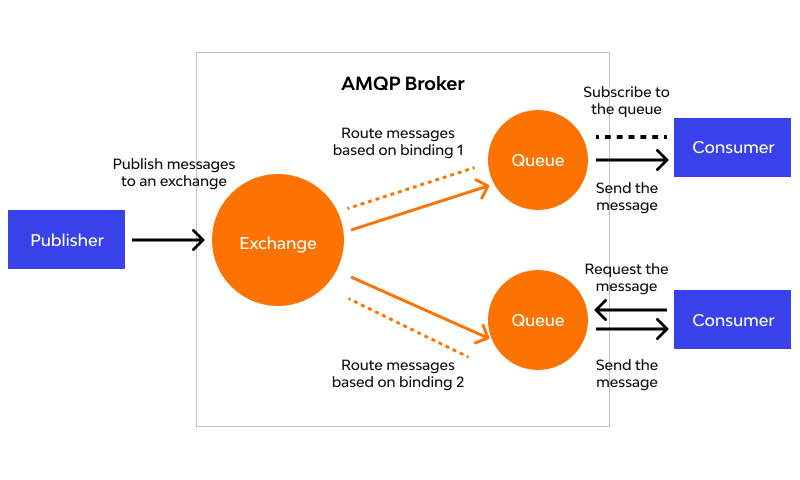
\includegraphics[width=0.9\textwidth,height=0.45\textheight,keepaspectratio]{assets/gambar/landasan-teori/amqp_model.png}%
  }{%
    \framebox[\textwidth][c]{\rule{0pt}{3.5cm}\parbox{0.82\textwidth}{\centering \textbf{[Placeholder Diagram: Model Pemetaan \textit{Exchange--Binding--Queue} AMQP 0-9-1]}\\\textit{Menampilkan Publisher $\rightarrow$ Exchange $\rightarrow$ Binding/Routing Key $\rightarrow$ Queues $\rightarrow$ Consumers. (Menunggu berkas gambar)}}}}
  \caption{Model Arsitektur Pemetaan \textit{Exchange--Binding--Queue} pada Protokol AMQP 0-9-1}
  \label{fig:teori_amqp}
\end{figure}

Sebagaimana terlihat pada Gambar~\ref{fig:teori_amqp}, produsen tidak mengirimkan pesan secara langsung ke antrean (\textit{queue}), melainkan menyerahkannya ke komponen \textit{exchange} disertai atribut \textit{routing key}. Selanjutnya, \textit{exchange} mengevaluasi aturan keterikatan (\textit{binding}) untuk menyalurkan pesan ke satu atau beberapa antrean tujuan sebelum dikonsumsi oleh konsumen~\cite{amqp_spec}. Jika pesan ditandai wajib terkirim (\textit{mandatory}) namun tidak ada antrean yang cocok, protokol mengembalikan pesan kepada pengirim melalui mekanisme \textit{BasicReturn}.

%------------------------------------------------------------
\section{RABBITMQ}
%------------------------------------------------------------

\textbf{RabbitMQ} merupakan implementasi \textit{message broker} sumber terbuka berbasis bahasa Erlang/OTP yang mengimplementasikan protokol AMQP 0-9-1 sebagai protokol utamanya serta mendukung protokol lain seperti STOMP dan MQTT melalui sistem plugin~\cite{rabbitmq_doc}. RabbitMQ menyediakan fitur keandalan operasional seperti persistensi antrean (\textit{durable queues}), konfirmasi penerbit (\textit{publisher confirms}), penampungan pesan gagal (\textit{dead-letter exchange}), serta kemampuan klastering untuk ketersediaan tinggi.

Dalam mengimplementasikan model AMQP, RabbitMQ menyediakan beberapa tipe \textit{exchange} yang disesuaikan dengan kebutuhan pola distribusi pesan pada sistem, sebagaimana ditunjukkan pada Gambar~\ref{fig:teori_rabbitmq_exchanges}.

\begin{figure}[H]
  \centering
  \IfFileExists{assets/gambar/landasan-teori/rabbitmq_direct_exchange.png}{%
    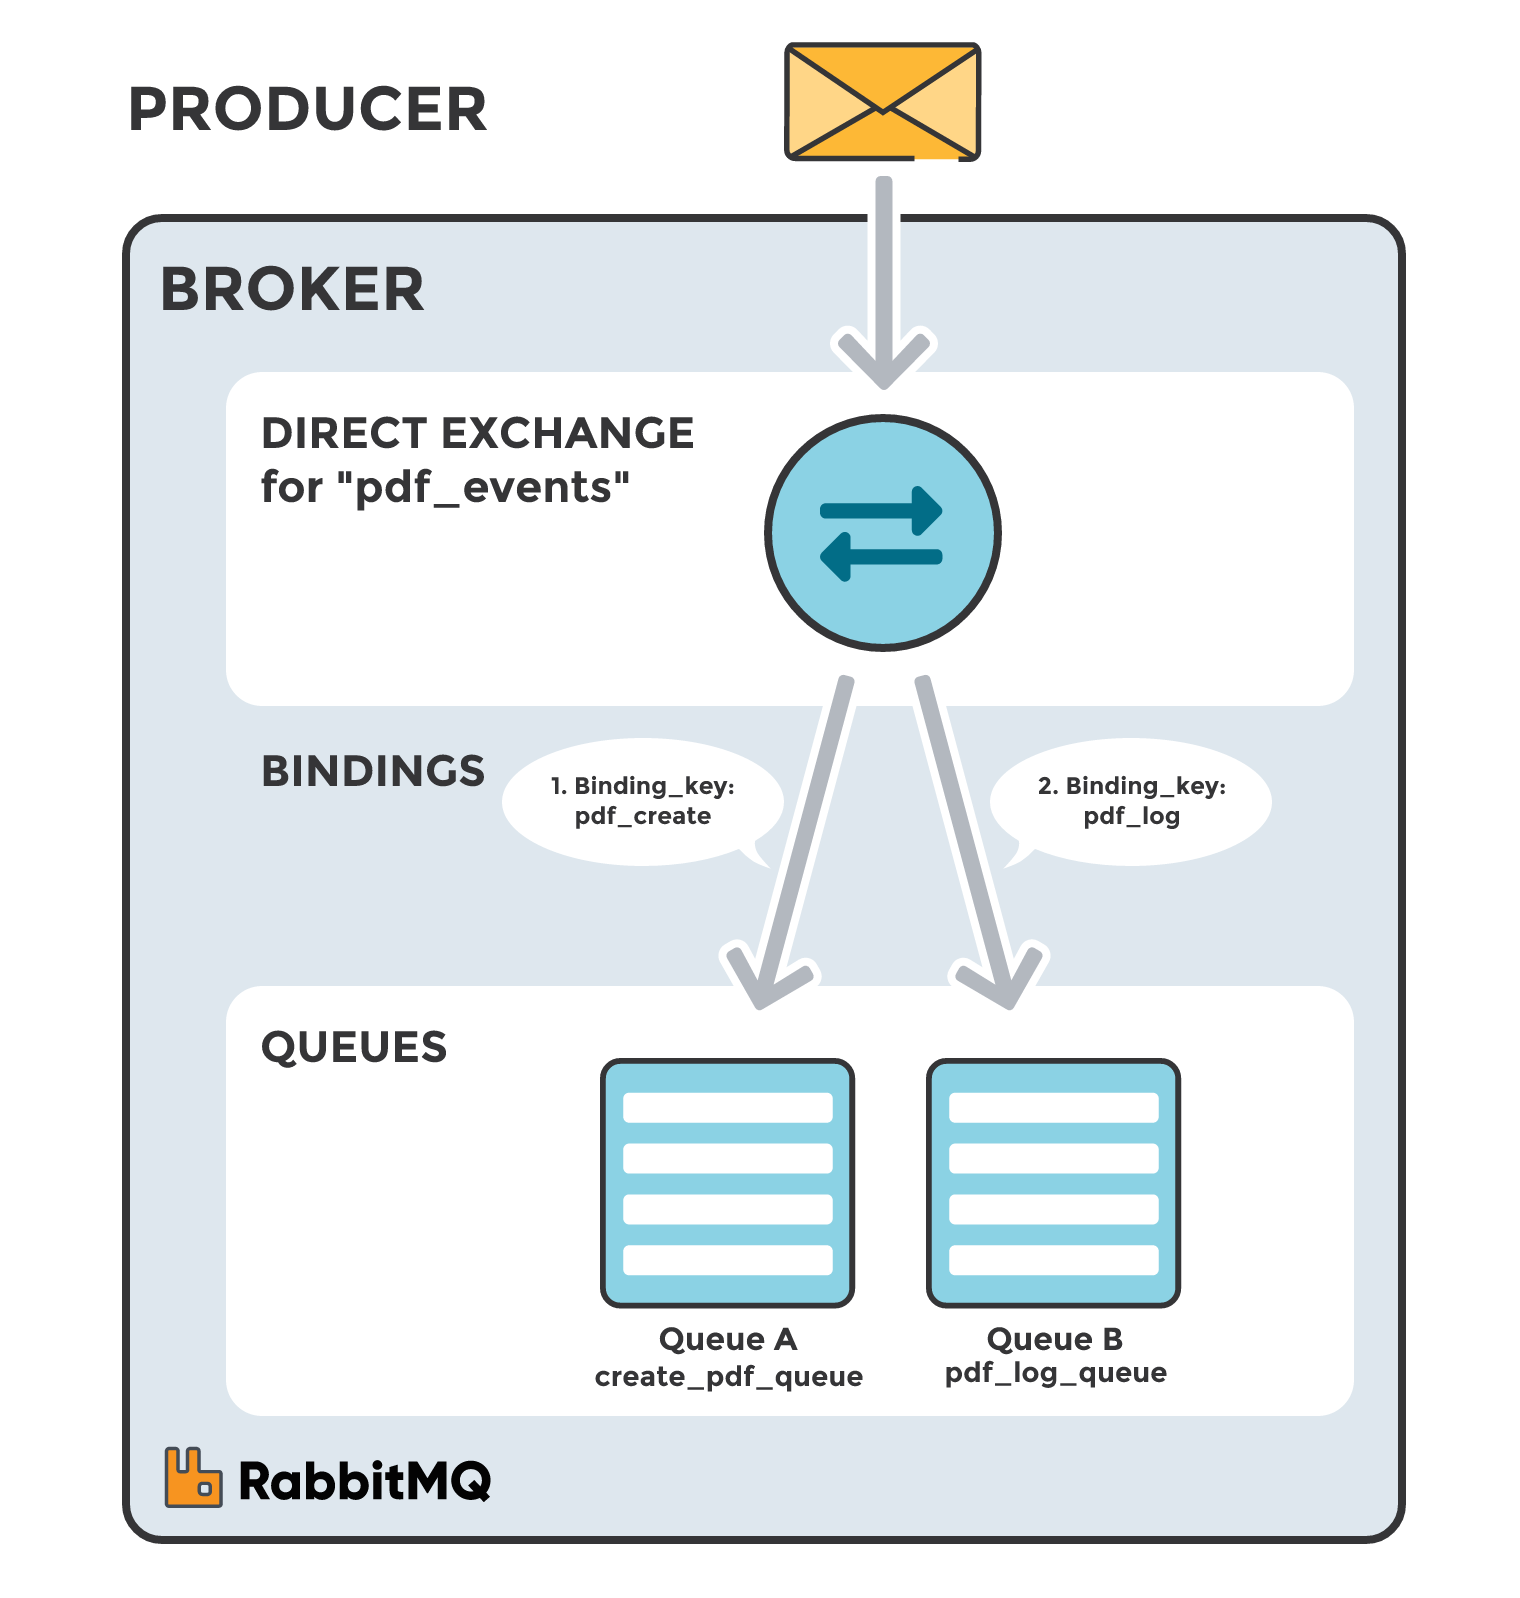
\includegraphics[width=0.45\textwidth,keepaspectratio]{assets/gambar/landasan-teori/rabbitmq_direct_exchange.png}\hspace{0.4cm}%
    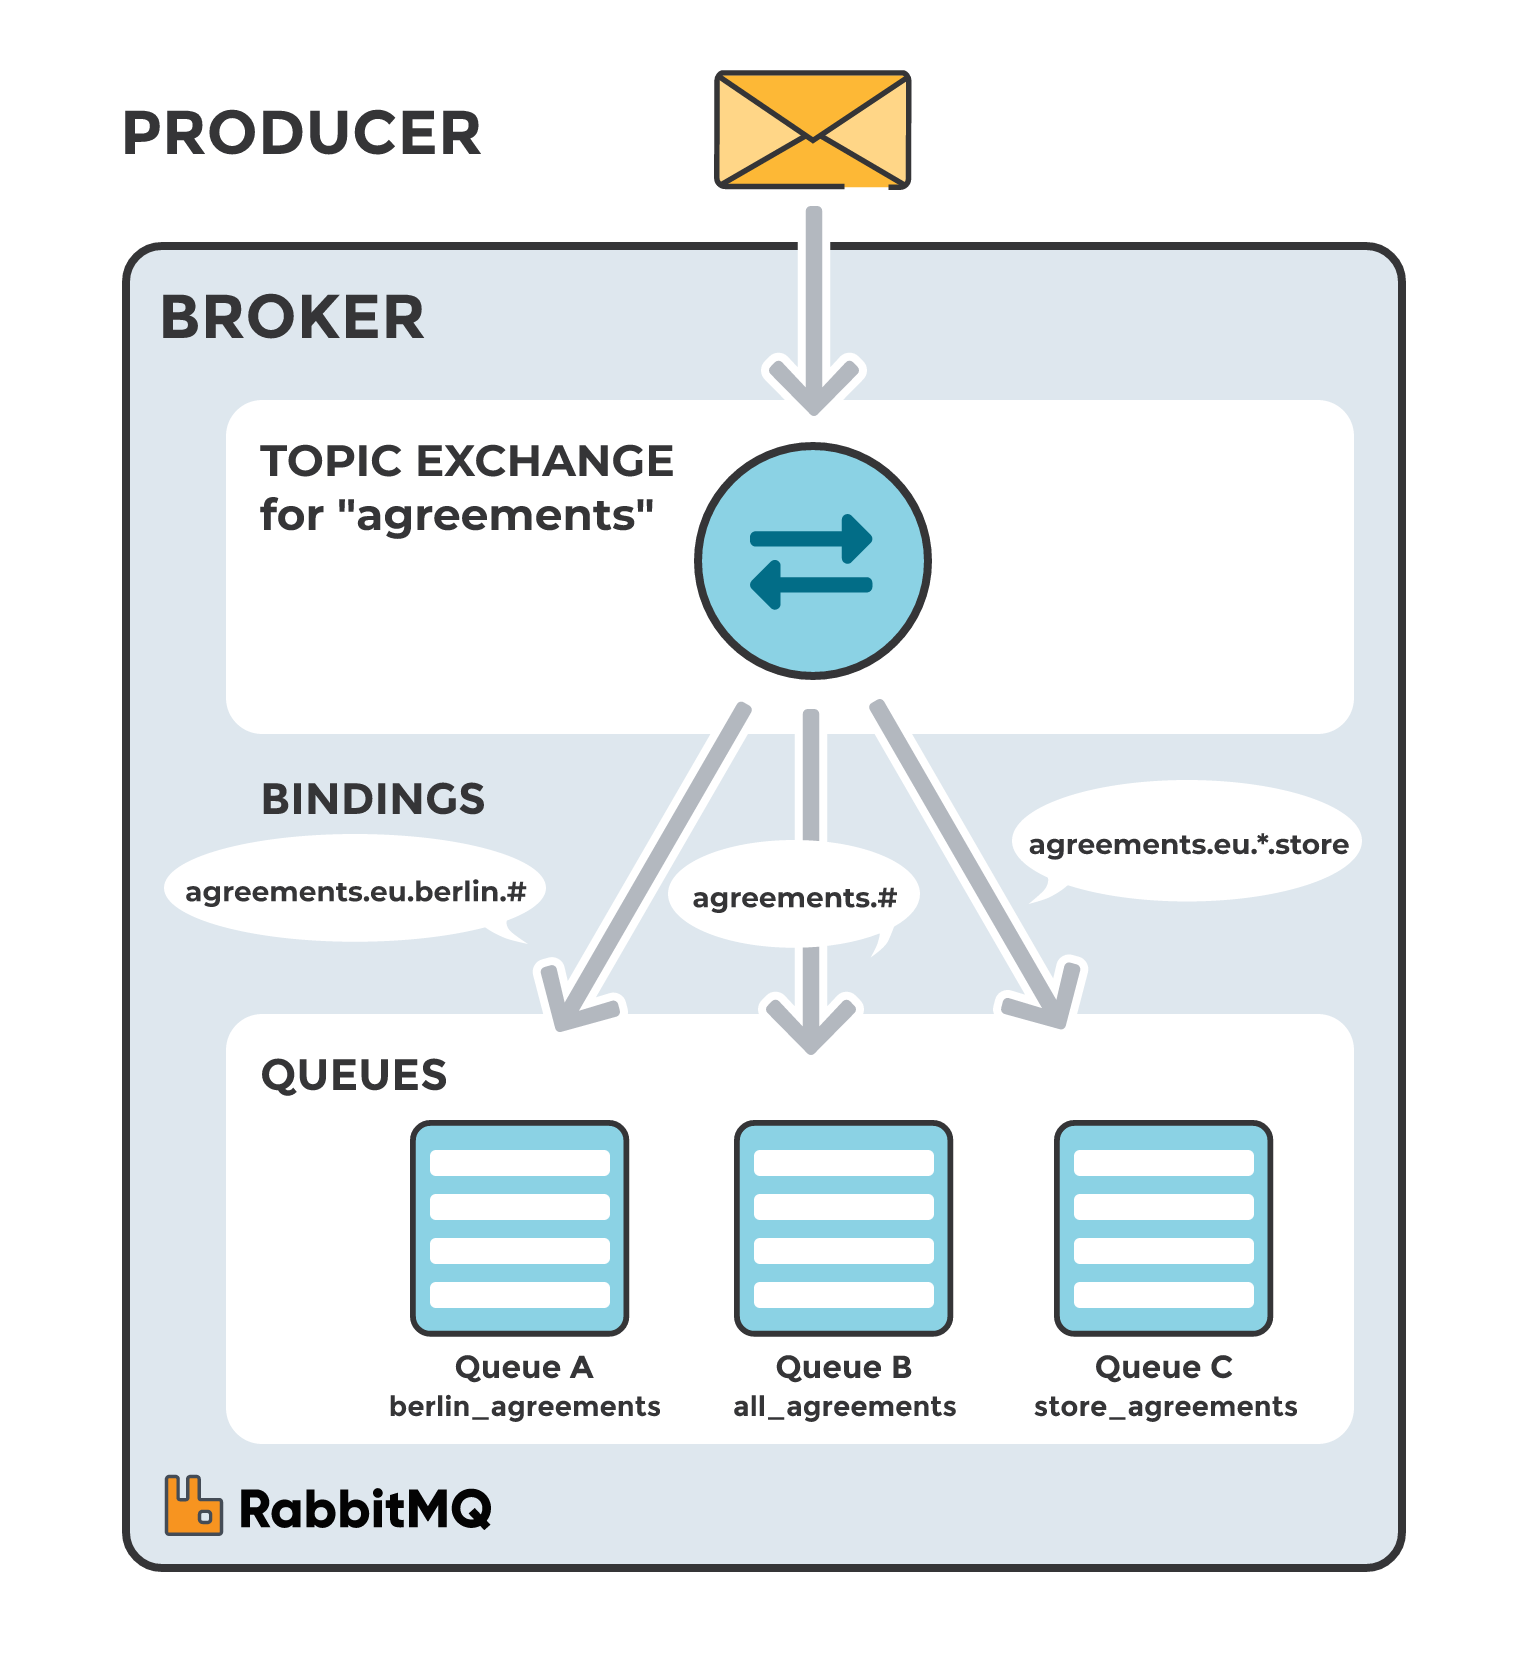
\includegraphics[width=0.45\textwidth,keepaspectratio]{assets/gambar/landasan-teori/rabbitmq_topic_exchange.png}\\[0.25cm]
    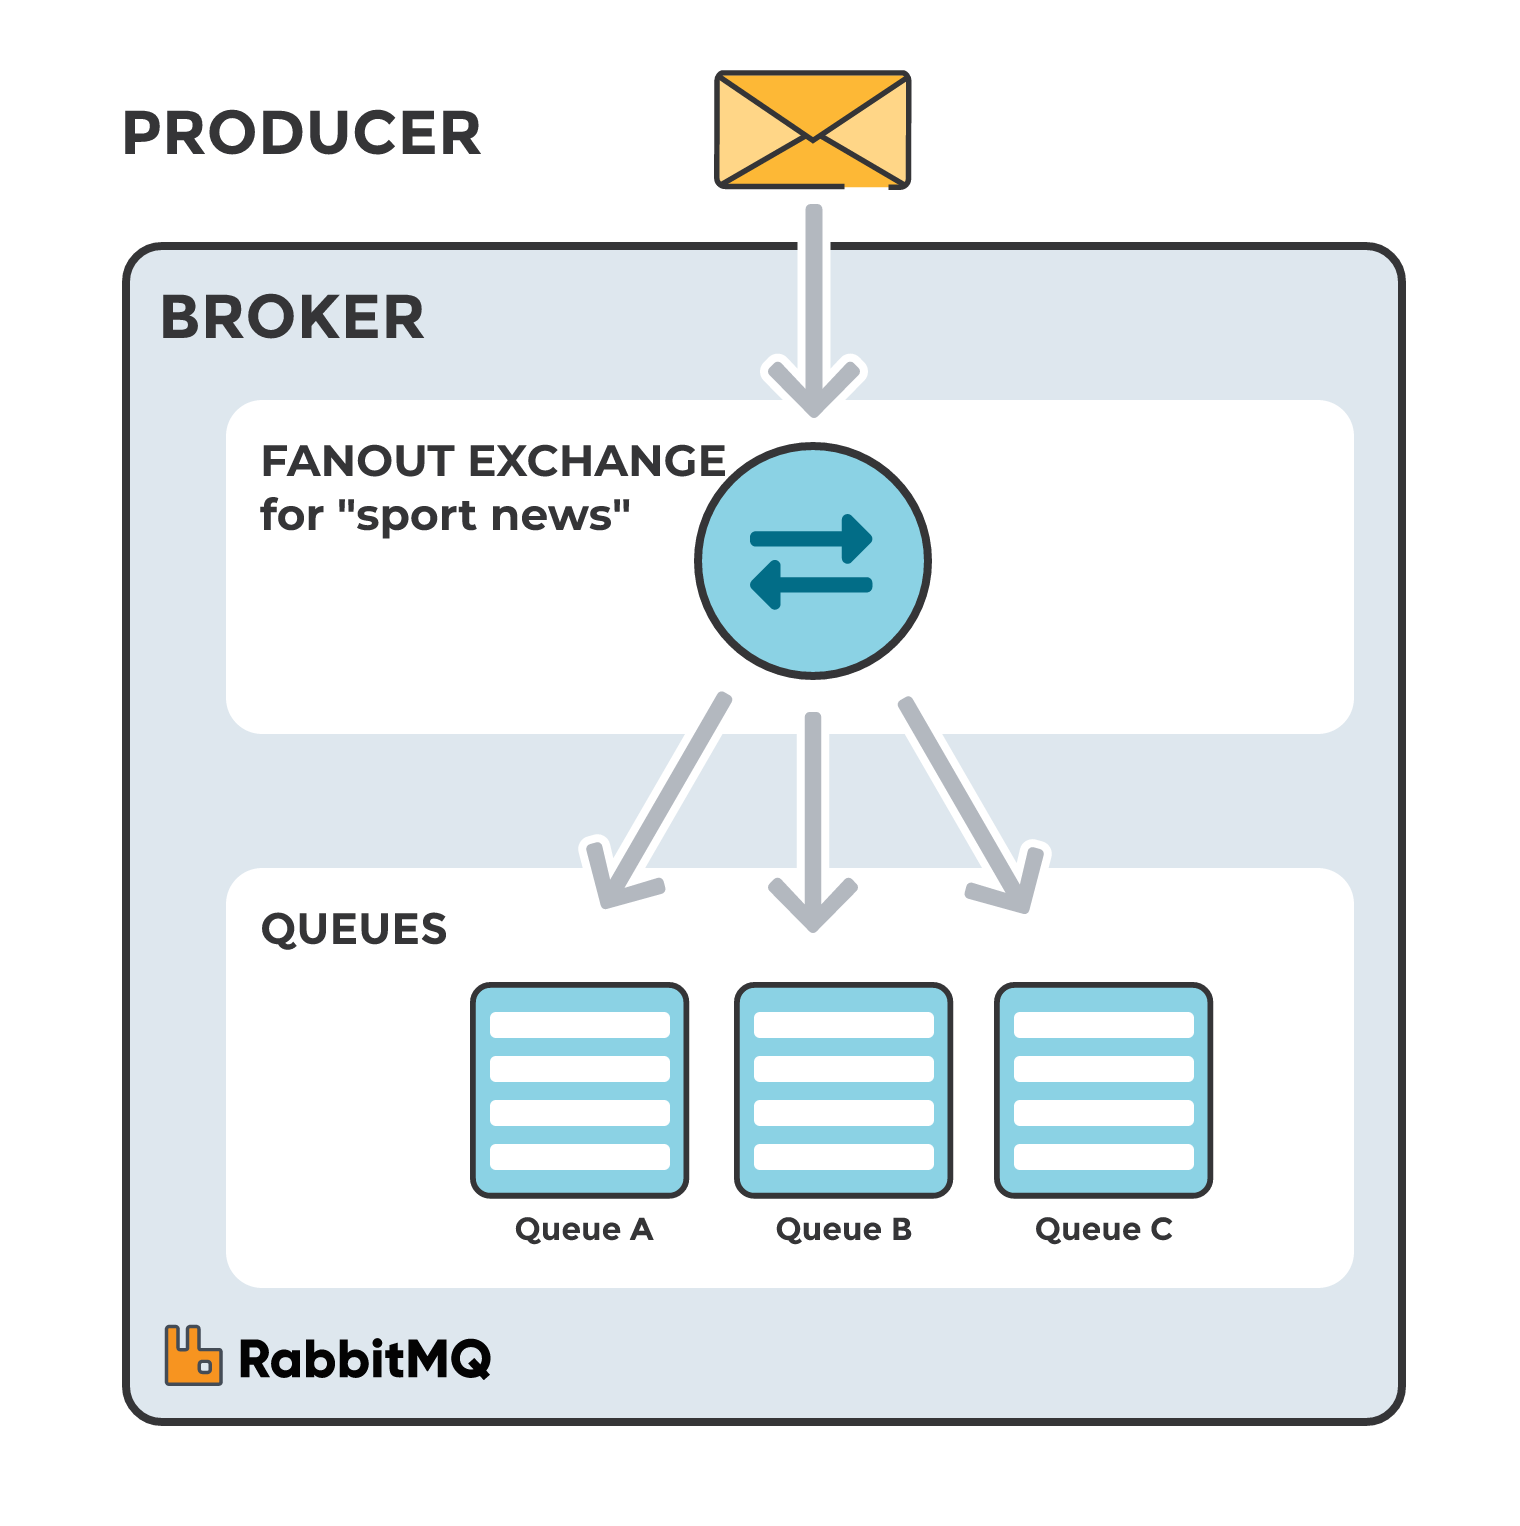
\includegraphics[width=0.45\textwidth,keepaspectratio]{assets/gambar/landasan-teori/rabbitmq_fanout_exchange.png}%
  }{%
    \framebox[\textwidth][c]{\rule{0pt}{3.5cm}\parbox{0.82\textwidth}{\centering \textbf{[Placeholder Diagram: Pola Perutean \textit{Direct}, \textit{Topic}, dan \textit{Fanout Exchange} RabbitMQ]}\\\textit{Menampilkan perbandingan perutean kunci persis, wildcard, dan broadcast ke seluruh antrean terikat. (Menunggu berkas gambar)}}}}
  \caption{Pola Perutean \textit{Direct}, \textit{Topic}, dan \textit{Fanout Exchange} pada RabbitMQ}
  \label{fig:teori_rabbitmq_exchanges}
\end{figure}

Mengacu pada Gambar~\ref{fig:teori_rabbitmq_exchanges}, proyek MonGrid memanfaatkan tiga jenis \textit{exchange} RabbitMQ sesuai karakteristik alur datanya: (1) \textbf{\textit{Direct Exchange}} untuk mengarahkan pesan ke antrean dengan \textit{routing key} yang identik (termasuk pola RPC asinkron dan deteksi pemutusan via \texttt{BasicReturn}); (2) \textbf{\textit{Topic Exchange}} pada \texttt{mongrid.update} untuk mendistribusikan pembaruan telemetri (\texttt{device.\{deviceId\}}) dan status alarm (\texttt{alarm.cleared}) berdasarkan pencocokan pola \textit{wildcard}; serta (3) \textbf{\textit{Fanout Exchange}} pada \texttt{hermes.control} untuk menyiarkan sinyal pembatalan aliran respons AI ke seluruh antrean terikat secara serentak~\cite{rabbitmq_doc}. Selain itu, plugin Web-STOMP pada RabbitMQ memungkinkan peramban web berlangganan topik \textit{exchange} secara langsung melalui WebSocket.

%------------------------------------------------------------
\section{PROTOKOL KOMUNIKASI WEBSOCKET}
%------------------------------------------------------------

\textbf{WebSocket} yang distandarkan dalam RFC 6455 adalah protokol komunikasi jaringan yang menyediakan saluran komunikasi dua arah penuh (\textit{full-duplex}) di atas satu koneksi TCP tunggal yang persisten~\cite{rfc6455_websocket}. Berbeda dari pola HTTP konvensional yang mewajibkan klien melakukan \textit{polling} atau \textit{long polling} berulang kali dengan muatan \textit{header} besar di setiap permintaan, WebSocket memungkinkan baik klien maupun server mengirimkan bingkai data (\textit{data frames}) kapan saja secara seketika dengan \textit{overhead} bingkai minimal (mulai dari 2 byte).

Proses pembentukan koneksi WebSocket dimulai dengan mekanisme \textit{HTTP Upgrade Handshake} melalui port standar HTTP (80/443) agar tetap kompatibel dengan infrastruktur proksi dan tembok api web, sebagaimana diilustrasikan pada Gambar~\ref{fig:teori_websocket}.

\begin{figure}[H]
  \centering
  \IfFileExists{assets/gambar/landasan-teori/websocket_handshake.png}{%
    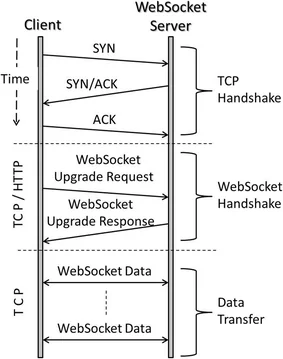
\includegraphics[width=0.88\textwidth,height=0.45\textheight,keepaspectratio]{assets/gambar/landasan-teori/websocket_handshake.png}%
  }{%
    \framebox[\textwidth][c]{\rule{0pt}{3.5cm}\parbox{0.82\textwidth}{\centering \textbf{[Placeholder Diagram: Mekanisme \textit{HTTP Upgrade Handshake} dan Komunikasi Dua Arah WebSocket]}\\\textit{Menampilkan urutan HTTP GET Upgrade $\rightarrow$ 101 Switching Protocols $\rightarrow$ Bidirectional Frames. (Menunggu berkas gambar)}}}}
  \caption{Mekanisme \textit{HTTP Upgrade Handshake} dan Komunikasi Dua Arah WebSocket}
  \label{fig:teori_websocket}
\end{figure}

Berdasarkan Gambar~\ref{fig:teori_websocket}, klien mengawali koneksi dengan mengirimkan permintaan HTTP \texttt{GET} berisi \textit{header} \texttt{Upgrade: websocket}, \texttt{Connection: Upgrade}, dan \texttt{Sec-WebSocket-Key}. Apabila server menyetujui, server membalas dengan kode status \texttt{101 Switching Protocols}, sehingga koneksi TCP yang sama langsung beralih menjadi saluran WebSocket persisten~\cite{rfc6455_websocket}. Pada proyek kerja praktik, WebSocket menjadi lapis transport bagi protokol STOMP pada dasbor pemantauan \textit{real-time} MonGrid serta menjadi saluran koneksi soket WhatsApp Web pada layanan Baileys PT Makassar Trans.

%------------------------------------------------------------
\section{PROTOKOL KOMUNIKASI STOMP}
%------------------------------------------------------------

\textbf{STOMP} (\textit{Simple/Streaming Text Oriented Messaging Protocol}) versi 1.2 adalah protokol perpesanan berbasis teks yang dirancang sederhana, ringan, dan mudah diimplementasikan lintas bahasa pemrograman di atas koneksi TCP maupun WebSocket~\cite{stomp_spec}. Berbeda dengan protokol biner seperti AMQP, format teks pada STOMP memudahkan proses inspeksi dan penelusuran kesalahan (\textit{debugging}) jaringan.

Setiap pesan dalam STOMP dikemas dalam struktur bingkai (\textit{frame}) yang diawali oleh baris perintah (\textit{command}), diikuti daftar pasangan kunci-nilai pada bagian \textit{header}, baris kosong, muatan isi (\textit{body}), dan diakhiri oleh karakter null (\texttt{\textbackslash0})~\cite{stomp_spec}. Perintah inti yang digunakan meliputi \texttt{CONNECT} untuk negosiasi sesi, \texttt{SEND} untuk mengirim pesan ke tujuan, \texttt{SUBSCRIBE} untuk berlangganan topik, \texttt{MESSAGE} untuk menerima dorongan data dari broker, serta \texttt{ACK} untuk konfirmasi pemrosesan. Pada MonGrid, antarmuka web berbasis React menggunakan pustaka \texttt{@stomp/stompjs} untuk membuka sesi STOMP over WebSocket langsung menuju plugin Web-STOMP RabbitMQ tanpa memerlukan layanan proksi tambahan~\cite{rabbitmq_doc, stomp_spec}.

%------------------------------------------------------------
\section{\textit{SERVER-SENT EVENTS} (SSE)}
%------------------------------------------------------------

\textbf{\textit{Server-Sent Events}} (SSE) adalah mekanisme standar HTML5/WHATWG yang memungkinkan server mendorong aliran pembaruan data secara searah (\textit{unidirectional server-push}) ke klien melalui koneksi HTTP standar tanpa memerlukan \textit{polling} berulang~\cite{mdn_sse}. Berbeda dengan WebSocket yang membangun protokol bingkai dua arah tersendiri, SSE bekerja di atas HTTP/1.1 maupun HTTP/2 dengan menetapkan tipe konten respons \texttt{text/event-stream} dan mempertahankan koneksi tetap terbuka.

Format aliran teks pada SSE disusun dari blok-blok baris berawalan \texttt{event:}, \texttt{data:}, \texttt{id:}, dan \texttt{retry:}. Di sisi peramban, antarmuka standar \texttt{EventSource} menyediakan kemampuan penyambungan ulang otomatis apabila koneksi terputus serta mengirimkan \textit{header} \texttt{Last-Event-ID} agar server dapat melanjutkan aliran peristiwa dari titik terakhir yang diterima klien~\cite{mdn_sse}. Mekanisme aliran data searah pada SSE diperlihatkan pada Gambar~\ref{fig:teori_sse}.

\begin{figure}[H]
  \centering
  \IfFileExists{assets/gambar/landasan-teori/server_sent_events.png}{%
    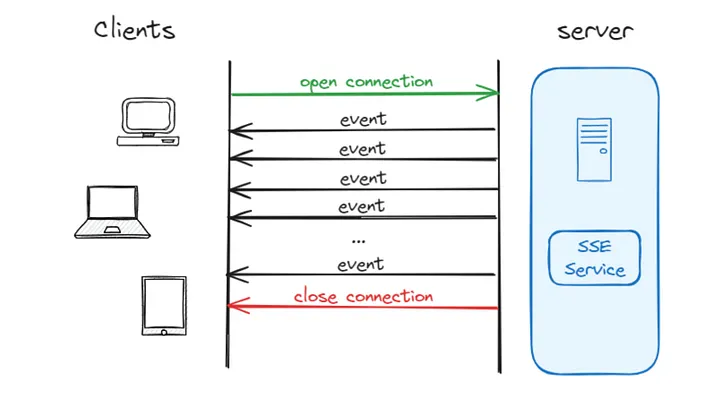
\includegraphics[width=0.88\textwidth,height=0.45\textheight,keepaspectratio]{assets/gambar/landasan-teori/server_sent_events.png}%
  }{%
    \framebox[\textwidth][c]{\rule{0pt}{3.5cm}\parbox{0.82\textwidth}{\centering \textbf{[Placeholder Diagram: Aliran Data Searah \textit{Server-Sent Events} (SSE)]}\\\textit{Menampilkan koneksi HTTP tunggal persisten dengan dorongan bertahap text/event-stream dan Last-Event-ID. (Menunggu berkas gambar)}}}}
  \caption{Aliran Data Searah \textit{Server-Sent Events} (SSE) Melalui Koneksi HTTP Persisten}
  \label{fig:teori_sse}
\end{figure}

Berdasarkan Gambar~\ref{fig:teori_sse}, sifatnya yang ringan dan searah menjadikan SSE sangat ideal untuk skenario \textit{streaming} keluaran teks dan telemetri dari server ke antarmuka web. Pada proyek kerja praktik, SSE dimanfaatkan untuk mengalirkan potongan token respons AI secara bertahap (\textit{token streaming}) pada modul AI Chat MonGrid serta mengalirkan jejak langkah penalaran dan konsumsi token agen secara langsung pada Nedo Agentic Platform.

%------------------------------------------------------------
\section{PROTOKOL KOMUNIKASI MQTT}
%------------------------------------------------------------

\textbf{MQTT} (\textit{Message Queuing Telemetry Transport}), yang distandarkan oleh OASIS pada versi 3.1.1 dan 5.0, adalah protokol komunikasi mesin-ke-mesin (\textit{M2M}) dan \textit{Internet of Things} (IoT) berbasis pola \textit{publish-subscribe} di atas TCP/IP~\cite{oasis_mqtt5, naik2017choice}. Dibandingkan protokol HTTP yang membawa \textit{header} teks berukuran besar di setiap permintaan, MQTT dirancang sangat ringan dengan ukuran \textit{header} tetap minimal 2 byte sehingga efisien untuk perangkat dengan keterbatasan daya maupun jaringan berbandwidth rendah dan tidak stabil~\cite{naik2017choice}.

Untuk menjamin keandalan pengiriman pesan sesuai kebutuhan aplikasi, spesifikasi MQTT menyediakan tiga tingkatan \textit{Quality of Service} (QoS) dengan alur jabat tangan paket yang ditunjukkan pada Gambar~\ref{fig:teori_mqtt_qos}.

\begin{figure}[H]
  \centering
  \IfFileExists{assets/gambar/landasan-teori/mqtt_qos_levels.png}{%
    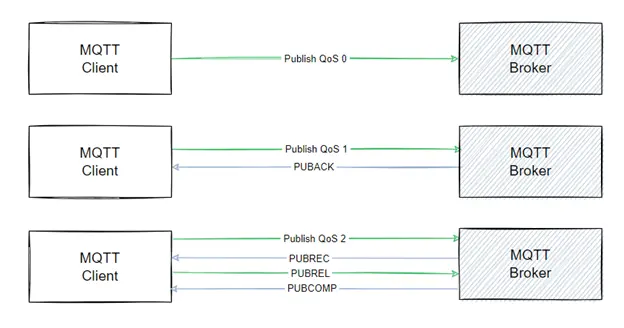
\includegraphics[width=0.92\textwidth,height=0.45\textheight,keepaspectratio]{assets/gambar/landasan-teori/mqtt_qos_levels.png}%
  }{%
    \framebox[\textwidth][c]{\rule{0pt}{3.5cm}\parbox{0.82\textwidth}{\centering \textbf{[Placeholder Diagram: Jabat Tangan Pengiriman Paket MQTT QoS 0, QoS 1, dan QoS 2]}\\\textit{Menampilkan alur PUBLISH (QoS 0), PUBLISH--PUBACK (QoS 1), dan 4-way handshake (QoS 2). (Menunggu berkas gambar)}}}}
  \caption{Mekanisme Jabat Tangan Pengiriman Pesan MQTT pada Tingkat QoS 0, QoS 1, dan QoS 2}
  \label{fig:teori_mqtt_qos}
\end{figure}

Mengacu pada Gambar~\ref{fig:teori_mqtt_qos}, QoS 0 (\textit{at most once}) mengirimkan paket \texttt{PUBLISH} sekali tanpa konfirmasi, QoS 1 (\textit{at least once}) memastikan pesan tiba minimal satu kali melalui konfirmasi \texttt{PUBACK}, sedangkan QoS 2 (\textit{exactly once}) menjamin pesan diterima tepat satu kali melalui jabat tangan empat langkah (\texttt{PUBLISH}, \texttt{PUBREC}, \texttt{PUBREL}, \texttt{PUBCOMP})~\cite{oasis_mqtt5, naik2017choice}. Selain itu, MQTT 5.0 menstandarkan fitur penamaan topik hierarkis dengan karakter \textit{wildcard} (\texttt{+} dan \texttt{\#}) serta \textit{shared subscription} (\texttt{\$share/<group>/<topic>}) guna mendistribusikan beban konsumsi ke banyak pekerja paralel, sebagaimana diterapkan pada akuisisi telemetri gardu MonGrid menggunakan QoS 1.

%------------------------------------------------------------
\section{EMQX}
%------------------------------------------------------------

\textbf{EMQX} adalah \textit{broker} MQTT terdistribusi sumber terbuka berkinerja tinggi berbasis Erlang/OTP yang dirancang untuk menangani konektivitas jutaan perangkat IoT secara bersamaan~\cite{emqx_doc}. EMQX mendukung penuh spesifikasi MQTT versi 3.1.1 dan 5.0 serta menyediakan kemampuan klastering lintas node untuk menjamin skalabilitas horizontal dan ketersediaan tinggi di lapisan penerimaan data.

Salah satu fitur krusial EMQX dalam arsitektur beban kerja tinggi adalah dukungan \textit{Shared Subscriptions} berbasis server untuk klien MQTT 3.1.1 maupun 5.0 melalui awalan topik \texttt{\$share/<group-name>/<topic>}~\cite{emqx_doc}. Dengan mekanisme ini, broker secara otomatis menyeimbangkan distribusi pesan masuk ke satu instans pekerja di dalam kelompok berlangganan menggunakan strategi seperti \textit{round-robin}, \textit{random}, atau \textit{hash}. Pada proyek MonGrid, EMQX berperan sebagai gerbang akuisisi terdepan (\textit{ingestion broker}) yang menerima paket dari ribuan perangkat \textit{power meter} dan sensor lapangan sebelum didistribusikan secara merata ke layanan \texttt{mongrid-producer}. Arsitektur EMQX dan mekanisme \textit{shared subscription} ditunjukkan pada Gambar~\ref{fig:teori_emqx}.

\begin{figure}[H]
  \centering
  \IfFileExists{assets/gambar/landasan-teori/emqx_architecture.png}{%
    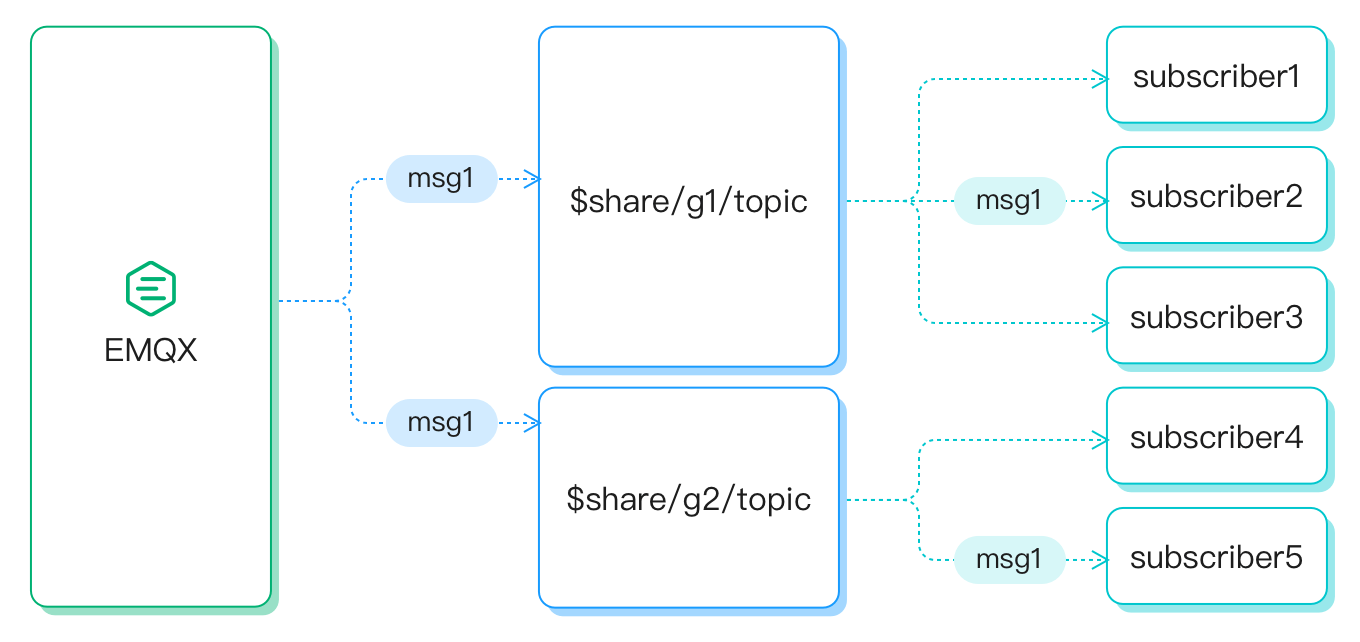
\includegraphics[width=0.9\textwidth,height=0.45\textheight,keepaspectratio]{assets/gambar/landasan-teori/emqx_architecture.png}%
  }{%
    \framebox[\textwidth][c]{\rule{0pt}{3.5cm}\parbox{0.82\textwidth}{\centering \textbf{[Placeholder Gambar: Arsitektur Broker MQTT EMQX dan \textit{Shared Subscriptions}]}\\\textit{Menunggu berkas gambar/diagram arsitektur resmi EMQX.}}}}
  \caption{Arsitektur Broker MQTT EMQX dan Mekanisme \textit{Shared Subscriptions}}
  \label{fig:teori_emqx}
\end{figure}

Berdasarkan Gambar~\ref{fig:teori_emqx}, broker EMQX menyalurkan pesan masuk (\texttt{msg1}) menuju dua kelompok langganan bersama yang berbeda, yaitu \texttt{\$share/g1/topic} (berisi \texttt{subscriber1} hingga \texttt{subscriber3}) dan \texttt{\$share/g2/topic} (berisi \texttt{subscriber4} dan \texttt{subscriber5}). Di dalam masing-masing kelompok, setiap pesan hanya dikirimkan ke tepat satu pelanggan aktif (misalnya \texttt{subscriber2} pada kelompok \texttt{g1} dan \texttt{subscriber5} pada kelompok \texttt{g2}), sehingga beban pemrosesan terbagi merata tanpa duplikasi eksekusi antarpekerja dalam satu kelompok.

%------------------------------------------------------------
\section{BASIS DATA RELASIONAL (RDBMS)}
%------------------------------------------------------------

Sistem manajemen basis data relasional (\textit{Relational Database Management System} / RDBMS) mengorganisasikan data ke dalam struktur relasi dua dimensi berupa tabel yang terdiri atas baris (\textit{tuple}) dan kolom (\textit{attribute}), dengan bahasa kueri deklaratif terstandarisasi SQL (\textit{Structured Query Language})~\cite{silberschatz2020database}. Hubungan antarentitas dijaga secara ketat melalui konstrain kunci primer (\textit{primary key}) dan kunci asing (\textit{foreign key}), serta ditata melalui proses normalisasi skema untuk menghindari anomali pembaruan dan redundansi data.

Untuk menjamin konsistensi dan integritas data pada eksekusi bersamaan maupun saat terjadi kegagalan sistem, RDBMS menegakkan empat properti transaksi yang dikenal sebagai \textbf{ACID}: \textit{Atomicity} (seluruh operasi transaksi berhasil atau dibatalkan menyeluruh), \textit{Consistency} (transaksi membawa basis data dari satu kondisi valid ke kondisi valid lainnya), \textit{Isolation} (eksekusi transaksi konkuren tidak saling mengganggu), dan \textit{Durability} (hasil transaksi yang telah dikomit tersimpan permanen)~\cite{silberschatz2020database}. Dalam sistem terdistribusi modern, RDBMS tetap memegang peran sentral sebagai sumber kebenaran utama (\textit{source of truth}) bagi data master dan transaksi bisnis.

%------------------------------------------------------------
\section{POSTGRESQL}
%------------------------------------------------------------

\textbf{PostgreSQL} adalah sistem manajemen basis data objek-relasional (\textit{Object-Relational Database Management System} / ORDBMS) sumber terbuka yang dikenal akan kepatuhan penuh terhadap standar SQL, ekstensibilitas tipe data, serta ketangguhannya dalam menangani konkurensi tinggi~\cite{postgresql_mvcc}. Untuk menjaga isolasi transaksi tanpa membuat operasi baca saling memblokir dengan operasi tulis, PostgreSQL mengimplementasikan model \textbf{\textit{Multi-Version Concurrency Control}} (MVCC), di mana setiap transaksi melihat potret (\textit{snapshot}) data yang konsisten pada titik waktu tertentu~\cite{postgresql_mvcc}.

Selain MVCC, PostgreSQL menyediakan fitur penguncian baris tingkat lanjut melalui klausa \texttt{SELECT ... FOR UPDATE SKIP LOCKED} serta penguncian transaksi \textit{advisory} (\texttt{pg\_advisory\_xact\_lock})~\cite{postgresql_locking}. Mekanisme penguncian baris non-blokir dengan klausa \texttt{SKIP LOCKED} diperlihatkan pada Gambar~\ref{fig:teori_postgres_skip_locked}.

\begin{figure}[H]
  \centering
  \IfFileExists{assets/gambar/landasan-teori/postgresql_skip_locked.png}{%
    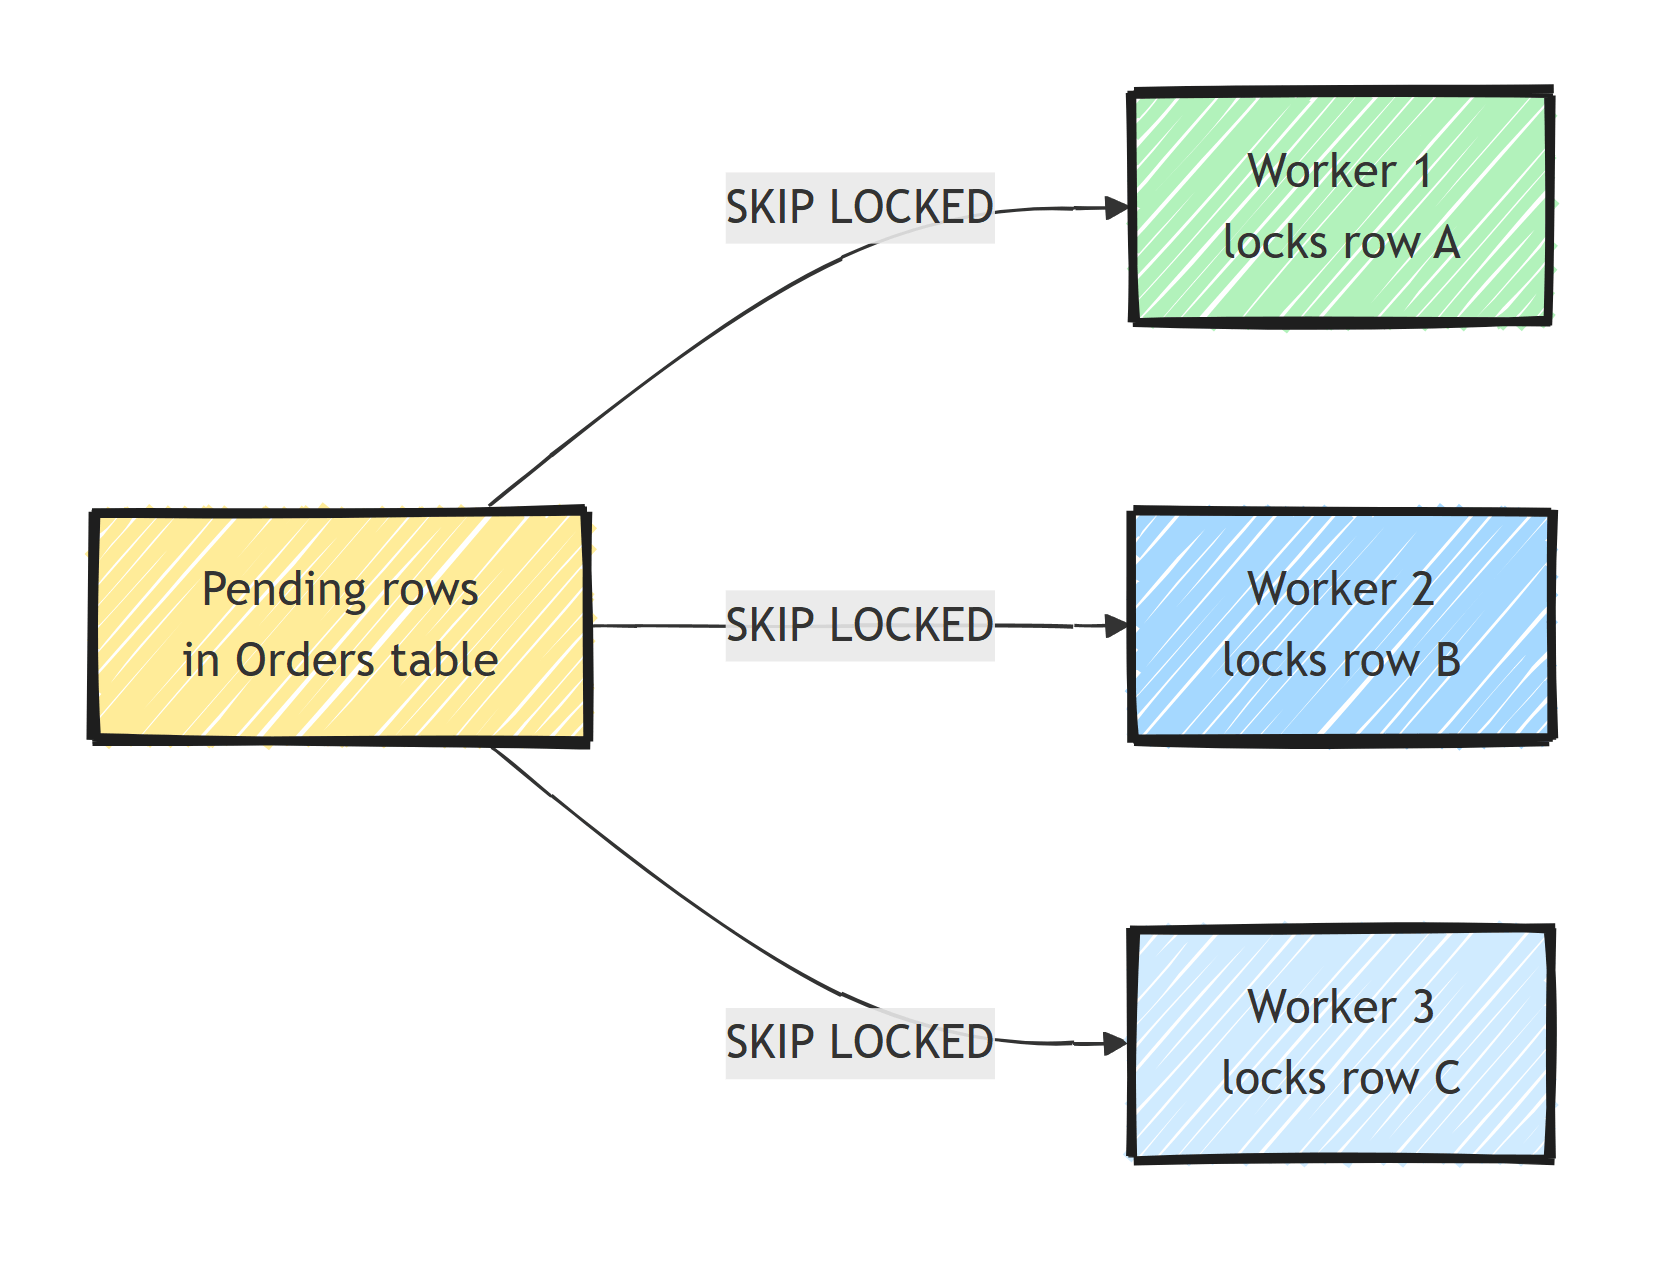
\includegraphics[width=0.9\textwidth,height=0.45\textheight,keepaspectratio]{assets/gambar/landasan-teori/postgresql_skip_locked.png}%
  }{%
    \framebox[\textwidth][c]{\rule{0pt}{3.5cm}\parbox{0.82\textwidth}{\centering \textbf{[Placeholder Diagram: Penguncian Baris Non-Blokir dengan \texttt{FOR UPDATE SKIP LOCKED}]}\\\textit{Menampilkan Worker 1 mengunci baris pertama dan Worker 2 melompati baris terkunci ke baris berikutnya. (Menunggu berkas gambar)}}}}
  \caption{Mekanisme Antrean Pekerja Konkuren dengan Klausa \texttt{FOR UPDATE SKIP LOCKED}}
  \label{fig:teori_postgres_skip_locked}
\end{figure}

Berdasarkan Gambar~\ref{fig:teori_postgres_skip_locked}, ketika beberapa pekerja mengakses tabel antrean secara bersamaan, baris yang sedang dikunci oleh transaksi pekerja lain langsung dilewati tanpa saling menunggu (\textit{non-blocking concurrency})~\cite{postgresql_locking}. Pada proyek kerja praktik, PostgreSQL digunakan sebagai basis data transaksional utama pada MonGrid (termasuk arsitektur dua tabel log alarm) dan menjadi fondasi mekanisme \textit{Transactional Job Leasing} anti-\textit{dual-write} pada Nedo Agentic Platform.

%------------------------------------------------------------
\section{MYSQL}
%------------------------------------------------------------

\textbf{MySQL} adalah sistem manajemen basis data relasional sumber terbuka yang mengadopsi arsitektur mesin penyimpanan modular (\textit{pluggable storage engine architecture}), memungkinkan pemilihan mekanisme penyimpanan fisik yang disesuaikan dengan karakteristik beban kerja aplikasi~\cite{mysql_innodb}. Pada rilis modern, mesin penyimpanan baku yang digunakan adalah \textbf{InnoDB}.

Mesin penyimpanan InnoDB menyediakan dukungan penuh terhadap transaksi ACID melalui mekanisme \textit{commit}, \textit{rollback}, dan pemulihan pasca-gangguan (\textit{crash recovery}), penguncian tingkat baris (\textit{row-level locking}) untuk mendukung akses tulis konkuren, serta penegakan integritas referensial \textit{foreign key} di level mesin basis data~\cite{mysql_innodb}. Selain itu, InnoDB menata tabel secara fisik menggunakan indeks klaster (\textit{clustered index}) berbasis struktur \textit{B+Tree} yang mempercepat pencarian berdasarkan kunci primer. Pada proyek PT Makassar Trans, MySQL digunakan untuk mengelola seluruh transaksi operasional tanda terima barang, rincian muatan (\textit{Bulk Input}), pencatatan status pemrosesan OCR, serta pelacakan status pengiriman dokumen.

%------------------------------------------------------------
\section{BASIS DATA \textit{IN-MEMORY}}
%------------------------------------------------------------

Basis data \textit{in-memory} (\textit{In-Memory Database} / IMDB) adalah sistem manajemen penyimpanan yang menempatkan keseluruhan atau himpunan data aktif langsung di dalam memori utama (RAM), alih-alih mengandalkan penyimpanan disk magnetik atau SSD sebagai jalur akses primer~\cite{kabakus2017performance}. Dengan mengeliminasi ketergantungan pada operasi masukan/keluaran (I/O) disk secara sinkron pada setiap pembacaan atau penulisan, basis data \textit{in-memory} mampu mencapai latensi akses dalam skala sub-milidetik serta \textit{throughput} yang jauh lebih tinggi dibandingkan RDBMS berbasis disk tradisional~\cite{kabakus2017performance}.

Perbandingan jalur akses data antara basis data berbasis disk tradisional dan basis data \textit{in-memory} ditunjukkan pada Gambar~\ref{fig:teori_in_memory}.

\begin{figure}[H]
  \centering
  \IfFileExists{assets/gambar/landasan-teori/disk_vs_in_memory.png}{%
    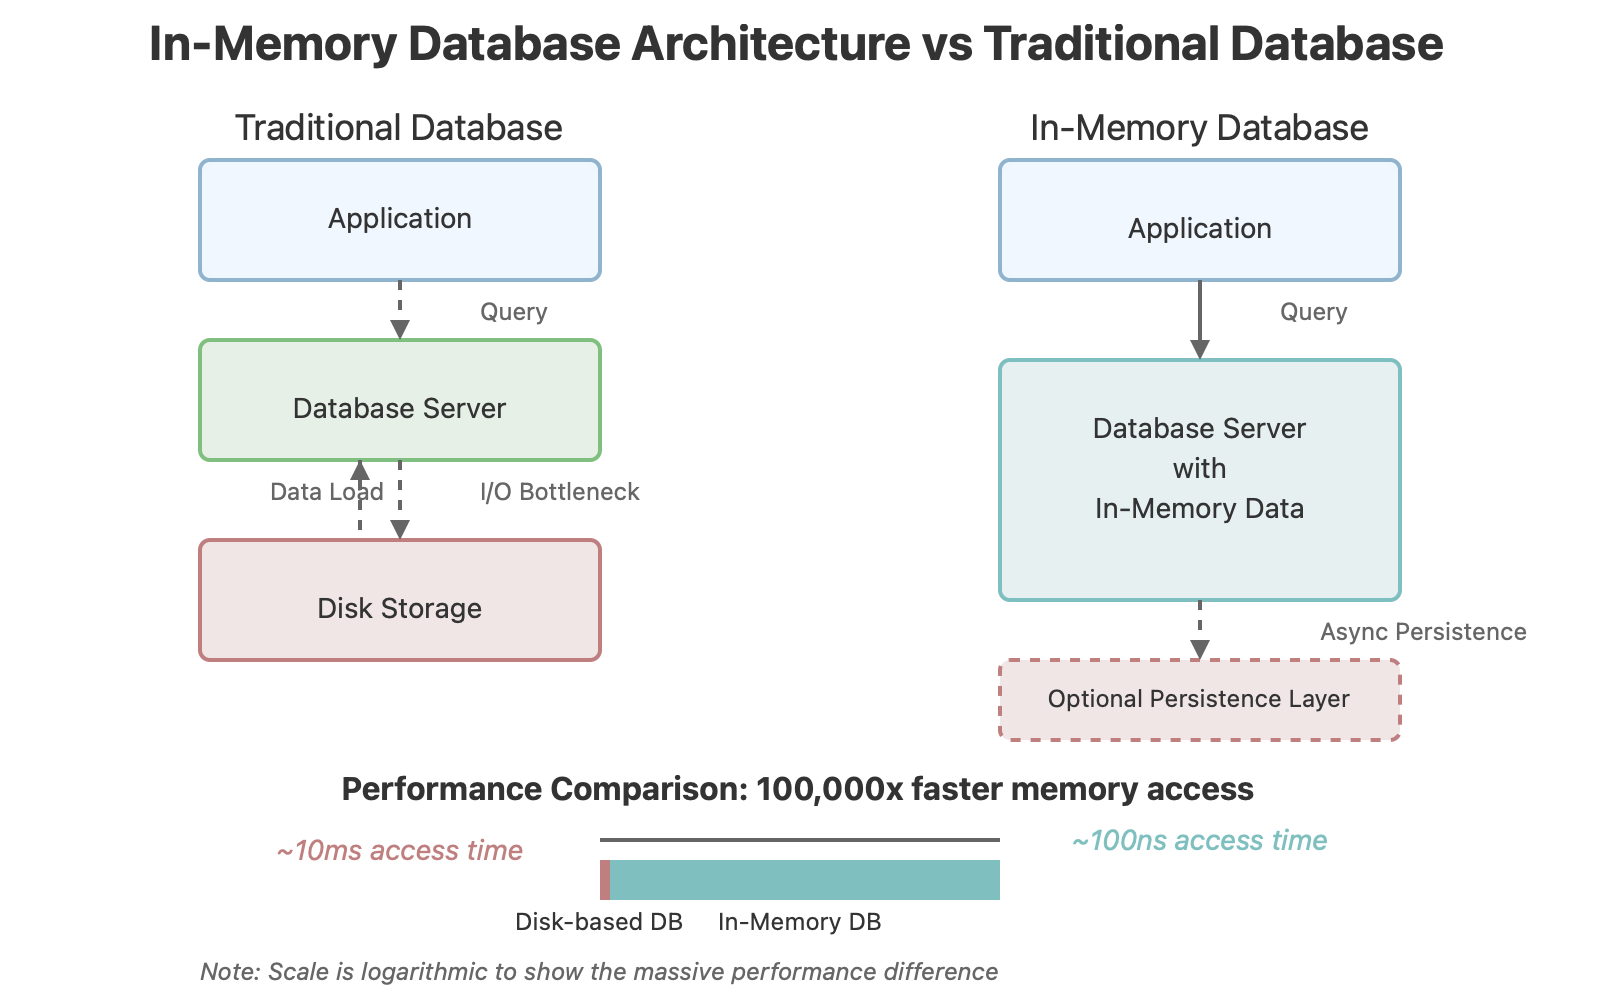
\includegraphics[width=0.9\textwidth,height=0.45\textheight,keepaspectratio]{assets/gambar/landasan-teori/disk_vs_in_memory.png}%
  }{%
    \framebox[\textwidth][c]{\rule{0pt}{3.5cm}\parbox{0.82\textwidth}{\centering \textbf{[Placeholder Diagram: Jalur Akses Data Basis Data Berbasis Disk vs \textit{In-Memory}]}\\\textit{Menampilkan perbandingan jalur I/O disk/page cache vs akses struktur data langsung di RAM. (Menunggu berkas gambar)}}}}
  \caption{Perbandingan Jalur Akses Data Basis Data Berbasis Disk dan Basis Data \textit{In-Memory}}
  \label{fig:teori_in_memory}
\end{figure}

Sebagaimana terlihat pada Gambar~\ref{fig:teori_in_memory}, efisiensi akses langsung di RAM menjadikan IMDB sangat cocok digunakan sebagai lapisan \textit{caching} berkecepatan tinggi, penyimpanan status sementara (\textit{transient state}), manajemen sesi, maupun pembatas laju permintaan (\textit{rate limiting}). Namun, karena sifat alami RAM yang volatil serta biaya kapasitas per gigabyte yang lebih tinggi dibanding disk, penerapannya umumnya dipadukan dengan basis data relasional atau deret waktu sebagai penyimpan persisten jangka panjang.

%------------------------------------------------------------
\section{REDIS}
%------------------------------------------------------------

\textbf{Redis} (\textit{Remote Dictionary Server}) adalah penyimpan struktur data \textit{in-memory} sumber terbuka yang beroperasi dengan arsitektur pemrosesan perintah \textit{single-threaded event loop} sehingga terhindar dari biaya pergantian konteks utas dan penguncian (\textit{lock contention}) pada struktur data inti~\cite{redis_doc, kabakus2017performance}. Berbeda dari penyimpan \textit{key-value} sederhana yang hanya menerima teks mentah, Redis mendukung beragam tipe struktur data tingkat lanjut secara natif, meliputi \textit{String}, \textit{Hash}, \textit{List}, \textit{Set}, \textit{Sorted Set}, dan \textit{Stream}, disertai mekanisme masa berlaku kunci otomatis (\textit{Time-To-Live} / TTL)~\cite{redis_doc}.

Untuk menjaga keamanan data dari kegagalan daya tanpa mengorbankan kecepatan di RAM, Redis menyediakan opsi persistensi hibrida berupa pengambilan potret berkala ke disk (\textit{RDB snapshot}) dan pencatatan log setiap operasi tulis (\textit{Append-Only File} / AOF)~\cite{redis_doc}. Pada proyek MonGrid, Redis berfungsi menyimpan status telemetri mutakhir (\textit{latest device state}), \textit{cache} pemetaan parameter meter, dan \textit{cache} aturan alarm sehingga evaluasi oleh \texttt{mongrid-consumer} berlangsung instan tanpa membebani PostgreSQL. Sementara itu, pada Nedo Agentic Platform, Redis dimanfaatkan sebagai broker pesan Celery, penyalur sinyal pembangun (\textit{wakeup hints}), dan saluran aliran telemetri eksekusi agen.

%------------------------------------------------------------
\section{BASIS DATA DERET WAKTU (\textit{TIME-SERIES})}
%------------------------------------------------------------

Basis data deret waktu (\textit{Time-Series Database} / TSDB) adalah sistem basis data yang dirancang khusus untuk menangani data yang terindeks dan berurutan berdasarkan penanda waktu (\textit{timestamp})~\cite{pelkonen2015gorilla}. Beban kerja data deret waktu—seperti metrik sistem dan telemetri sensor kelistrikan—memiliki karakteristik khas, yaitu dominasi penulisan berfrekuensi tinggi secara berurutan ke akhir deret (\textit{append-only}), hampir tidak pernah dimutakhirkan kembali, serta kueri analitik yang umumnya memindai rentang jendela waktu tertentu untuk agregasi tren.

Untuk mencapai efisiensi ruang dan kecepatan kueri pada skala masif, TSDB menerapkan partisi data berbasis rentang waktu, teknik kompresi numerik khusus seperti \textit{delta-of-delta} untuk \textit{timestamp} dan kompresi XOR (\textit{Gorilla compression}) untuk nilai titik mengambang~\cite{pelkonen2015gorilla}, serta mekanisme kebijakan retensi (\textit{retention policy}) dan penurunan resolusi (\textit{downsampling/rollup}). Konsep retensi dan \textit{downsampling} bertingkat ditunjukkan pada Gambar~\ref{fig:teori_tsdb_downsample}.

\begin{figure}[H]
  \centering
  \IfFileExists{assets/gambar/landasan-teori/timeseries_downsampling.png}{%
    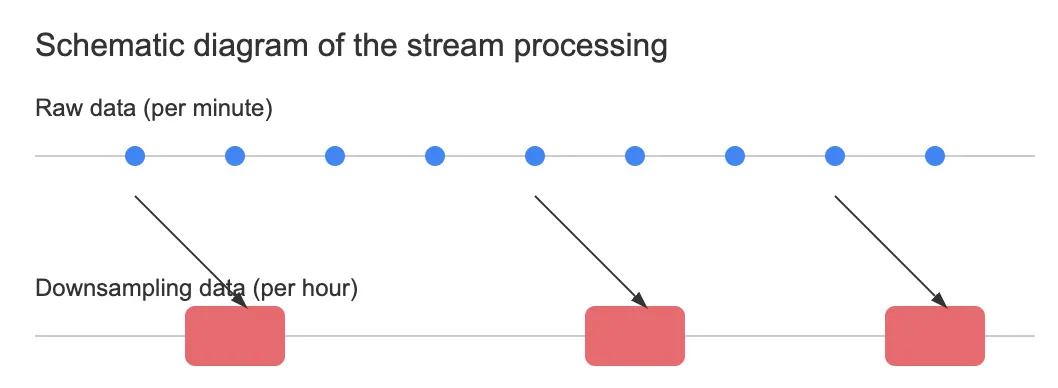
\includegraphics[width=0.9\textwidth,height=0.45\textheight,keepaspectratio]{assets/gambar/landasan-teori/timeseries_downsampling.png}%
  }{%
    \framebox[\textwidth][c]{\rule{0pt}{3.5cm}\parbox{0.82\textwidth}{\centering \textbf{[Placeholder Diagram: Konsep \textit{Downsampling} dan Retensi Data Deret Waktu Bertingkat]}\\\textit{Menampilkan transformasi data mentah beresolusi tinggi ke data agregat jangka panjang. (Menunggu berkas gambar)}}}}
  \caption{Konsep \textit{Downsampling} dan Retensi Data Deret Waktu Bertingkat}
  \label{fig:teori_tsdb_downsample}
\end{figure}

Berdasarkan Gambar~\ref{fig:teori_tsdb_downsample}, data mentah beresolusi detik hanya disimpan dalam jangka pendek untuk pemantauan detail, sedangkan ringkasan statistiknya (rata-rata, minimum, maksimum) disimpan dalam resolusi yang lebih kasar untuk analisis historis jangka panjang tanpa membengkakkan kapasitas disk.

%------------------------------------------------------------
\section{INFLUXDB}
%------------------------------------------------------------

\textbf{InfluxDB} adalah basis data deret waktu sumber terbuka yang dioptimalkan untuk menerima, mengompresi, dan menganalisis data metrik serta telemetri IoT berfrekuensi tinggi~\cite{influxdb_downsample}. Dalam model datanya, InfluxDB mengelompokkan titik data ke dalam wadah bernama \textit{bucket}, yang di dalamnya terdiri atas \textit{measurement} (setara nama tabel logis), \textit{tag} (pasangan kunci-nilai metadata yang diindeks seperti \texttt{device\_id}), \textit{field} (nilai pengukuran numerik yang tidak diindeks), serta \textit{timestamp} presisi tinggi.

Proses penulisan data ke InfluxDB menggunakan format teks ringan bernama \textit{Line Protocol}, yang kemudian disimpan secara efisien di disk oleh mesin penyimpanan \textit{Time-Structured Merge Tree} (TSM)~\cite{influxdb_downsample}. Pada proyek MonGrid, InfluxDB menjadi penyimpanan historis utama seluruh telemetri sensor gardu, di mana tugas latar belakang \texttt{InfluxDbRollupTask} menjalankan strategi \textit{cascading downsampling} dari resolusi mentah (\texttt{raw}) hingga bulanan (\texttt{1M}) dengan jendela tumpang-tindih untuk menampung paket data yang tiba terlambat~\cite{influxdb_downsample}. Anatomi format \textit{Line Protocol} dan struktur data InfluxDB ditunjukkan pada Gambar~\ref{fig:teori_influxdb}.

\begin{figure}[H]
  \centering
  \IfFileExists{assets/gambar/landasan-teori/influxdb_line_protocol.png}{%
    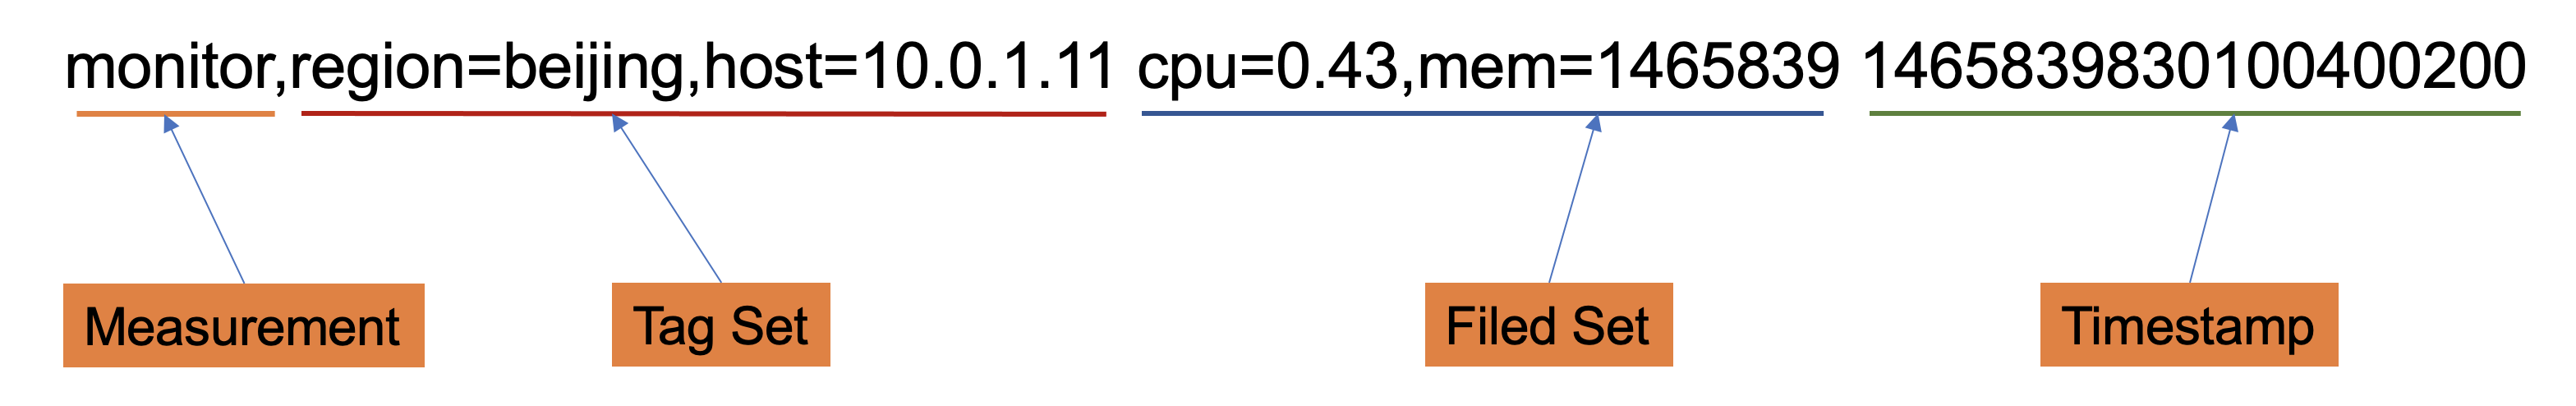
\includegraphics[width=0.9\textwidth,height=0.45\textheight,keepaspectratio]{assets/gambar/landasan-teori/influxdb_line_protocol.png}%
  }{%
    \framebox[\textwidth][c]{\rule{0pt}{3.5cm}\parbox{0.82\textwidth}{\centering \textbf{[Placeholder Gambar: Anatomi Format \textit{Line Protocol} dan Struktur Data InfluxDB]}\\\textit{Menunggu berkas gambar/diagram resmi dokumentasi InfluxData.}}}}
  \caption{Anatomi Format \textit{Line Protocol} dan Struktur Data InfluxDB}
  \label{fig:teori_influxdb}
\end{figure}

Mengacu pada Gambar~\ref{fig:teori_influxdb}, satu baris data \textit{Line Protocol} InfluxDB (\texttt{monitor,region=beijing,host=10.0.1.11 cpu=0.43,mem=1465839 1465839830100400200}) tersusun atas empat bagian utama yang dipisahkan koma dan spasi: \textit{Measurement} (\texttt{monitor}) sebagai nama kelompok metrik, \textit{Tag Set} (\texttt{region=beijing,host=10.0.1.11}) sebagai pasangan kunci-nilai metadata yang terindeks, \textit{Field Set} (\texttt{cpu=0.43,mem=1465839}) sebagai nilai data aktual yang dicatat, serta \textit{Timestamp} (\texttt{1465839830100400200}) sebagai penanda waktu berpresisi nanodetik.

%------------------------------------------------------------
\section{PENYIMPANAN OBJEK (\textit{OBJECT STORAGE})}
%------------------------------------------------------------

Penyimpanan objek (\textit{object storage}) adalah paradigma arsitektur penyimpanan yang mengelola data tidak terstruktur—seperti citra, dokumen PDF, rekaman video, dan arsip biner—sebagai unit mandiri bernama objek di dalam ruang nama datar (\textit{flat namespace}), tanpa hierarki direktori pohon maupun pengalamatan blok fisik konvensional~\cite{factor2005object}. Setiap objek mengemas tiga elemen utama: data biner mentah (\textit{payload}), metadata kaya yang dapat dikustomisasi secara bebas, serta pengenal unik global (\textit{object key/ID}).

Perbedaan mendasar antara paradigma \textit{file storage}, \textit{block storage}, dan \textit{object storage} diilustrasikan pada Gambar~\ref{fig:teori_object_storage}.

\begin{figure}[H]
  \centering
  \IfFileExists{assets/gambar/landasan-teori/storage_comparison.png}{%
    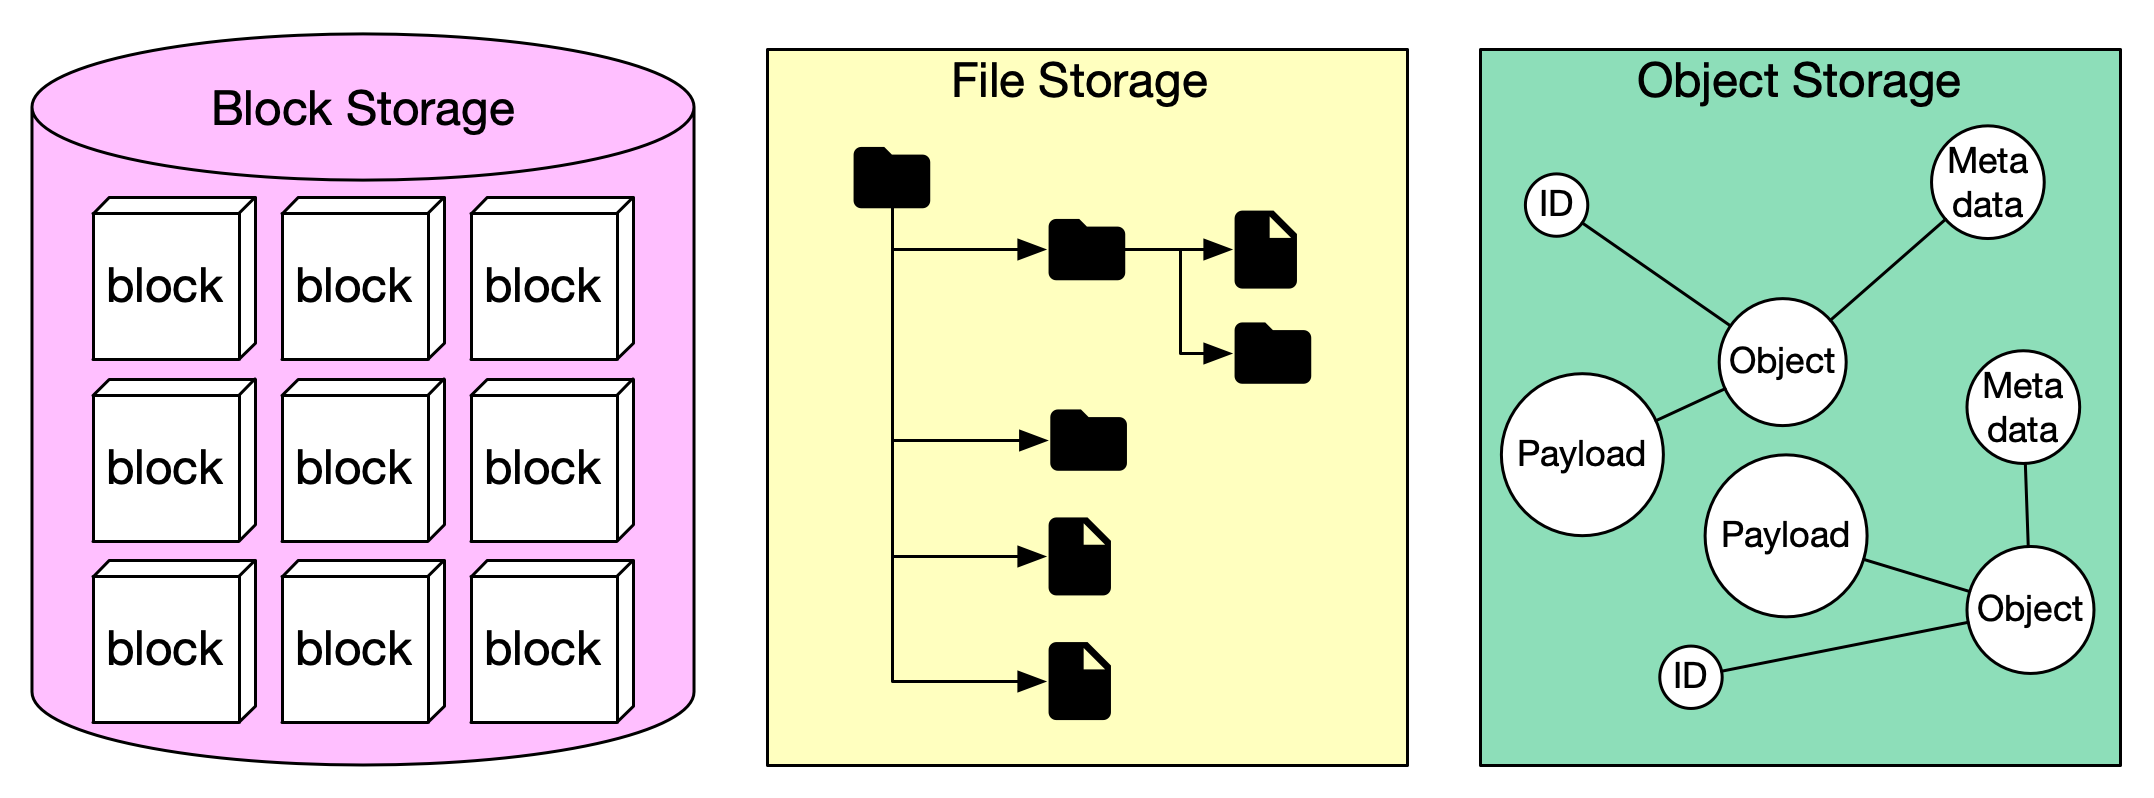
\includegraphics[width=0.92\textwidth,height=0.45\textheight,keepaspectratio]{assets/gambar/landasan-teori/storage_comparison.png}%
  }{%
    \framebox[\textwidth][c]{\rule{0pt}{3.5cm}\parbox{0.82\textwidth}{\centering \textbf{[Placeholder Diagram: Perbandingan \textit{File Storage}, \textit{Block Storage}, dan \textit{Object Storage}]}\\\textit{Menampilkan hierarki direktori (File), blok mentah (Block), dan wadah objek datar berbasis HTTP (Object). (Menunggu berkas gambar)}}}}
  \caption{Perbandingan Struktur \textit{File Storage}, \textit{Block Storage}, dan \textit{Object Storage}}
  \label{fig:teori_object_storage}
\end{figure}

Berdasarkan Gambar~\ref{fig:teori_object_storage}, pengaksesan objek melalui antarmuka protokol HTTP/REST (dengan Amazon S3 API sebagai standar \textit{de facto} industri) memudahkan skalabilitas kapasitas secara horizontal lintas layanan terdistribusi serta memisahkan penyimpanan berkas biner berukuran besar dari basis data relasional transaksional~\cite{factor2005object}.

%------------------------------------------------------------
\section{MINIO}
%------------------------------------------------------------

\textbf{MinIO} adalah peladen penyimpanan objek berkinerja tinggi sumber terbuka yang kompatibel penuh dengan antarmuka pemrograman Amazon S3 serta dirancang untuk dapat dijalankan secara mandiri (\textit{self-hosted}) pada infrastruktur lokal maupun kontainer~\cite{minio_doc}. Pengelolaan sumber daya pada MinIO mengorganisasikan objek ke dalam wadah logis bernama \textit{bucket}, dilengkapi manajemen kebijakan akses IAM, penerbitan tautan akses sementara yang ditandatangani (\textit{presigned URL}), serta perlindungan integritas data tingkat lanjut seperti \textit{erasure coding} dan proteksi \textit{bitrot}~\cite{minio_doc}.

Pada proyek PT Makassar Trans, MinIO memisahkan penyimpanan berkas biner (foto tanda terima asli, hasil pemotongan citra, dan dokumen PDF) dari metadata relasional yang dikelola aplikasi web~\cite{minio_doc}. Sementara itu, pada Nedo Agentic Platform, MinIO dimanfaatkan untuk menyimpan artefak luaran kerja agen dan arsip \textit{snapshot} ruang kerja terkompresi (\texttt{.tar.gz}) agar eksekusi tugas dapat berpindah lintas kontainer \textit{runner} secara portabel.

%------------------------------------------------------------
\section{ASP.NET CORE}
%------------------------------------------------------------

\textbf{ASP.NET Core} adalah kerangka kerja pengembangan aplikasi web dan layanan REST API lintas platform yang bersifat sumber terbuka dari Microsoft dan berjalan di atas platform .NET (digunakan versi .NET 9 pada proyek MonGrid)~\cite{aspnet_middleware, dotnet_background}. Kerangka kerja ini dirancang modular dengan performa tinggi serta menyediakan kontainer \textit{Dependency Injection} (DI) bawaan dan sistem konfigurasi terstruktur untuk mengelola siklus hidup komponen aplikasi secara terpusat.

Alur penanganan permintaan HTTP pada ASP.NET Core disusun sebagai rangkaian komponen \textit{middleware} yang membentuk sebuah saluran pipa pemrosesan (\textit{request pipeline}), di mana setiap komponen dapat memeriksa, memodifikasi, atau meneruskan permintaan ke komponen berikutnya sebelum menghasilkan respons~\cite{aspnet_middleware}. Alur pemrosesan pada \textit{middleware pipeline} ASP.NET Core diperlihatkan pada Gambar~\ref{fig:teori_aspnet_middleware}.

\begin{figure}[H]
  \centering
  \IfFileExists{assets/gambar/landasan-teori/aspnet_middleware_pipeline.png}{%
    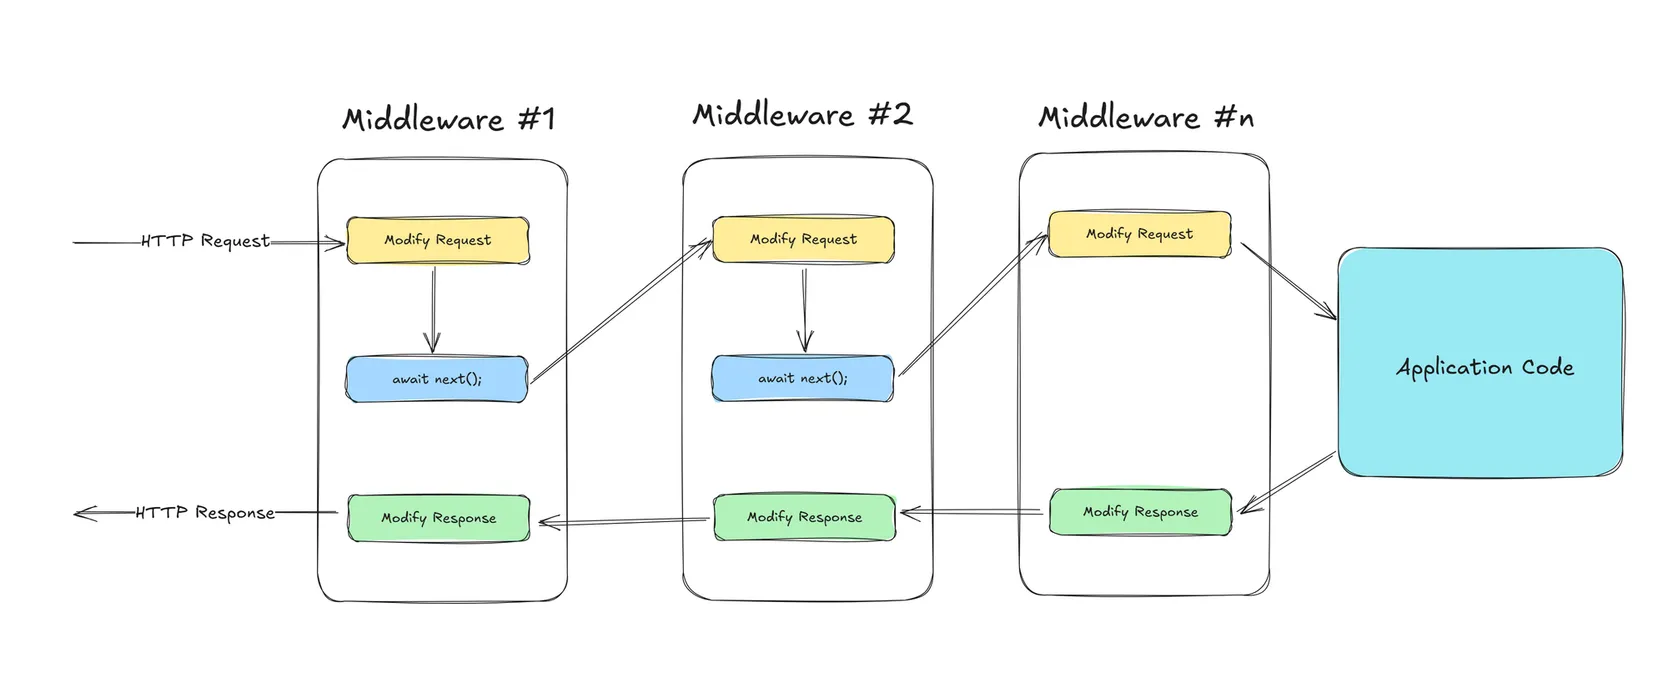
\includegraphics[width=0.9\textwidth,height=0.45\textheight,keepaspectratio]{assets/gambar/landasan-teori/aspnet_middleware_pipeline.png}%
  }{%
    \framebox[\textwidth][c]{\rule{0pt}{3.5cm}\parbox{0.82\textwidth}{\centering \textbf{[Placeholder Gambar: Alur \textit{Middleware Request Pipeline} pada ASP.NET Core]}\\\textit{Menunggu berkas gambar/diagram resmi dokumentasi Microsoft Learn.}}}}
  \caption{Alur Pemrosesan Permintaan melalui \textit{Middleware Pipeline} pada ASP.NET Core}
  \label{fig:teori_aspnet_middleware}
\end{figure}

Berdasarkan Gambar~\ref{fig:teori_aspnet_middleware}, setiap \textit{HTTP Request} yang masuk mula-mula diproses oleh \textit{Middleware \#1} (\textit{Modify Request}), lalu diteruskan secara berurutan melalui pemanggilan \texttt{await next();} ke \textit{Middleware \#2} hingga \textit{Middleware \#n} sampai mencapai \textit{Application Code} sebagai penangan akhir. Setelah itu, \textit{HTTP Response} yang dihasilkan mengalir kembali dalam urutan terbalik melewati blok \textit{Modify Response} pada setiap komponen sebelum dikirimkan kepada klien, sehingga fungsi lintas aspek seperti autentikasi, pencatatan log, dan penanganan galat dapat diterapkan secara terpusat.

\subsection{\textit{Hosted Service} dan \texttt{BackgroundService}}

Untuk menjalankan proses pekerja latar belakang jangka panjang di luar siklus permintaan-respons HTTP—seperti pemrosesan antrean pesan atau penjadwalan agregasi berkala—ekosistem .NET menyediakan antarmuka \texttt{IHostedService} dan kelas abstrak \texttt{BackgroundService}~\cite{dotnet_background}. Komponen ini dikelola langsung oleh siklus hidup \textit{host} aplikasi serta mendukung penghentian anggun (\textit{graceful shutdown}) melalui \texttt{CancellationToken}. Pada proyek MonGrid, pola ini menjadi fondasi layanan tanpa kepala (\textit{headless services}) pada \texttt{mongrid-producer}, \texttt{mongrid-consumer}, dan \texttt{mongrid-bgservice} (\texttt{DataSyncTask} serta \texttt{InfluxDbRollupTask}).

%------------------------------------------------------------
\section{FLASK}
%------------------------------------------------------------

\textbf{Flask} adalah \textit{microframework} aplikasi web berbasis bahasa Python yang dibangun di atas perangkat antarmuka WSGI \textbf{Werkzeug} dan mesin templat \textbf{Jinja2}~\cite{flask_doc}. Berbeda dari kerangka kerja monolitik yang memaksakan konvensi ORM atau struktur proyek tertentu sejak awal, Flask mengusung inti yang ramping namun mudah diperluas (\textit{extensible}), dilengkapi mekanisme perutean URL (\textit{routing}), konteks permintaan terisolasi (\textit{request/application context}), serta fitur \textbf{\textit{Blueprint}} untuk memecah aplikasi berskala besar ke dalam modul-modul fungsional yang rapi~\cite{flask_doc}.

Pada lingkungan produksi yang melayani banyak koneksi aliran data berdurasi panjang (\textit{streaming}), Flask dapat dipadukan dengan pekerja asinkron WSGI seperti \texttt{gevent} guna menghindari pemblokiran utas utama. Pada Nedo Agentic Platform, Flask menjadi kerangka kerja tulang punggung layanan REST API inti, penyaji titik akhir aliran telemetri SSE, serta implementasi \textit{Nedo LLM Gateway} (\texttt{/api/llm/v1}).

%------------------------------------------------------------
\section{PYTHON \texttt{ASYNCIO}}
%------------------------------------------------------------

\textbf{\texttt{asyncio}} adalah pustaka standar pada Python untuk menulis kode pemrograman konkuren menggunakan sintaks \texttt{async/await} di atas model \textit{single-threaded event loop}~\cite{python_asyncio}. Berbeda dari \textit{multithreading} di Python yang kerap terbatasi oleh \textit{Global Interpreter Lock} (GIL) pada tugas komputasi CPU maupun menanggung beban pergantian konteks utas sistem operasi, \texttt{asyncio} menerapkan \textit{cooperative multitasking}: saat sebuah \textit{coroutine} menunggu operasi I/O jaringan selesai, kendali eksekusi langsung diserahkan ke \textit{event loop} untuk menjalankan \textit{Task} atau \textit{Future} lainnya~\cite{python_asyncio}.

Pendekatan kooperatif ini mencapai efisiensi sangat tinggi untuk beban kerja yang didominasi oleh latensi jaringan (\textit{I/O-bound}). Pada Nedo Agentic Platform, \texttt{asyncio} menjadi fondasi utama mesin eksekusi agen mandiri (\texttt{nedo.runner.engine}) untuk mengorkestrasi komunikasi paralel menuju \textit{Nedo LLM Gateway}, basis data, dan layanan mikro MCP secara nir-blokir.

%------------------------------------------------------------
\section{CELERY}
%------------------------------------------------------------

\textbf{Celery} adalah sistem antrean tugas terdistribusi (\textit{distributed task queue}) asinkron untuk ekosistem Python yang dirancang untuk memproses pekerjaan berdurasi lama di latar belakang secara terpisah dari siklus permintaan HTTP~\cite{celery_doc}. Arsitektur Celery membagi tanggung jawab ke dalam beberapa komponen independen: aplikasi pengirim tugas (\textit{Client}), perantara pesan (\textit{Message Broker} seperti Redis atau RabbitMQ), proses pekerja pengeksekusi (\textit{Celery Worker}), penyimpan hasil (\textit{Result Backend}), serta penjadwal tugas berkala (\textit{Celery Beat}) yang memicu pekerjaan sesuai jadwal \textit{cron} atau interval waktu tertentu~\cite{celery_doc}.

Interaksi antarkomponen dalam arsitektur sistem antrean tugas terdistribusi Celery diperlihatkan pada Gambar~\ref{fig:teori_celery}.

\begin{figure}[H]
  \centering
  \IfFileExists{assets/gambar/landasan-teori/celery_architecture.png}{%
    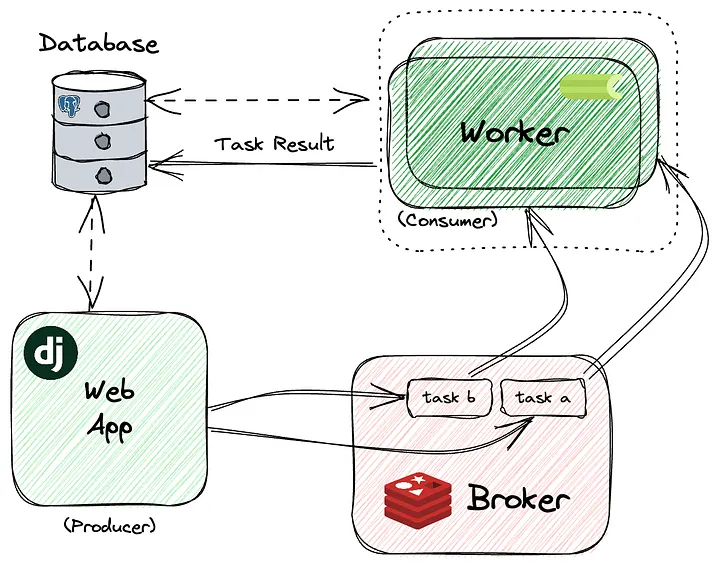
\includegraphics[width=0.9\textwidth,height=0.45\textheight,keepaspectratio]{assets/gambar/landasan-teori/celery_architecture.png}%
  }{%
    \framebox[\textwidth][c]{\rule{0pt}{3.5cm}\parbox{0.82\textwidth}{\centering \textbf{[Placeholder Diagram: Arsitektur Komponen Sistem Antrean Tugas Celery]}\\\textit{Menampilkan Client/Celery Beat $\rightarrow$ Message Broker (Redis) $\rightarrow$ Celery Workers $\rightarrow$ Result Backend. (Menunggu berkas gambar)}}}}
  \caption{Arsitektur Komponen Sistem Antrean Tugas Terdistribusi Celery}
  \label{fig:teori_celery}
\end{figure}

Sebagaimana diilustrasikan pada Gambar~\ref{fig:teori_celery}, selain eksekusi tugas tunggal, Celery menyediakan primitif komposisi alur kerja (\textit{Canvas}) seperti \textit{chain} dan \textit{group} untuk merangkai eksekusi bertahap~\cite{celery_doc}. Pada Nedo Agentic Platform, Celery menangani penjadwalan tugas pemeliharaan rutin (\textit{sweepers} pemulihan sewa tugas kedaluwarsa), pembuatan faktur PDF, pengiriman surel, serta orkestrasi alur kerja multi-agen berbasis DAG.

%------------------------------------------------------------
\section{\textit{JSON WEB TOKEN} (JWT)}
%------------------------------------------------------------

\textbf{\textit{JSON Web Token}} (JWT) yang distandarkan dalam RFC 7519 adalah format token ringkas dan aman-URL (\textit{URL-safe}) untuk merepresentasikan klaim identitas dan otorisasi antara dua pihak yang ditandatangani secara kriptografis~\cite{rfc7519_jwt}. Dalam format \textit{Compact Serialization}, sebuah JWT terdiri atas tiga segmen teks terenkode Base64URL yang dipisahkan oleh karakter titik, sebagaimana ditunjukkan pada Gambar~\ref{fig:teori_jwt}.

\begin{figure}[H]
  \centering
  \IfFileExists{assets/gambar/landasan-teori/jwt_structure.png}{%
    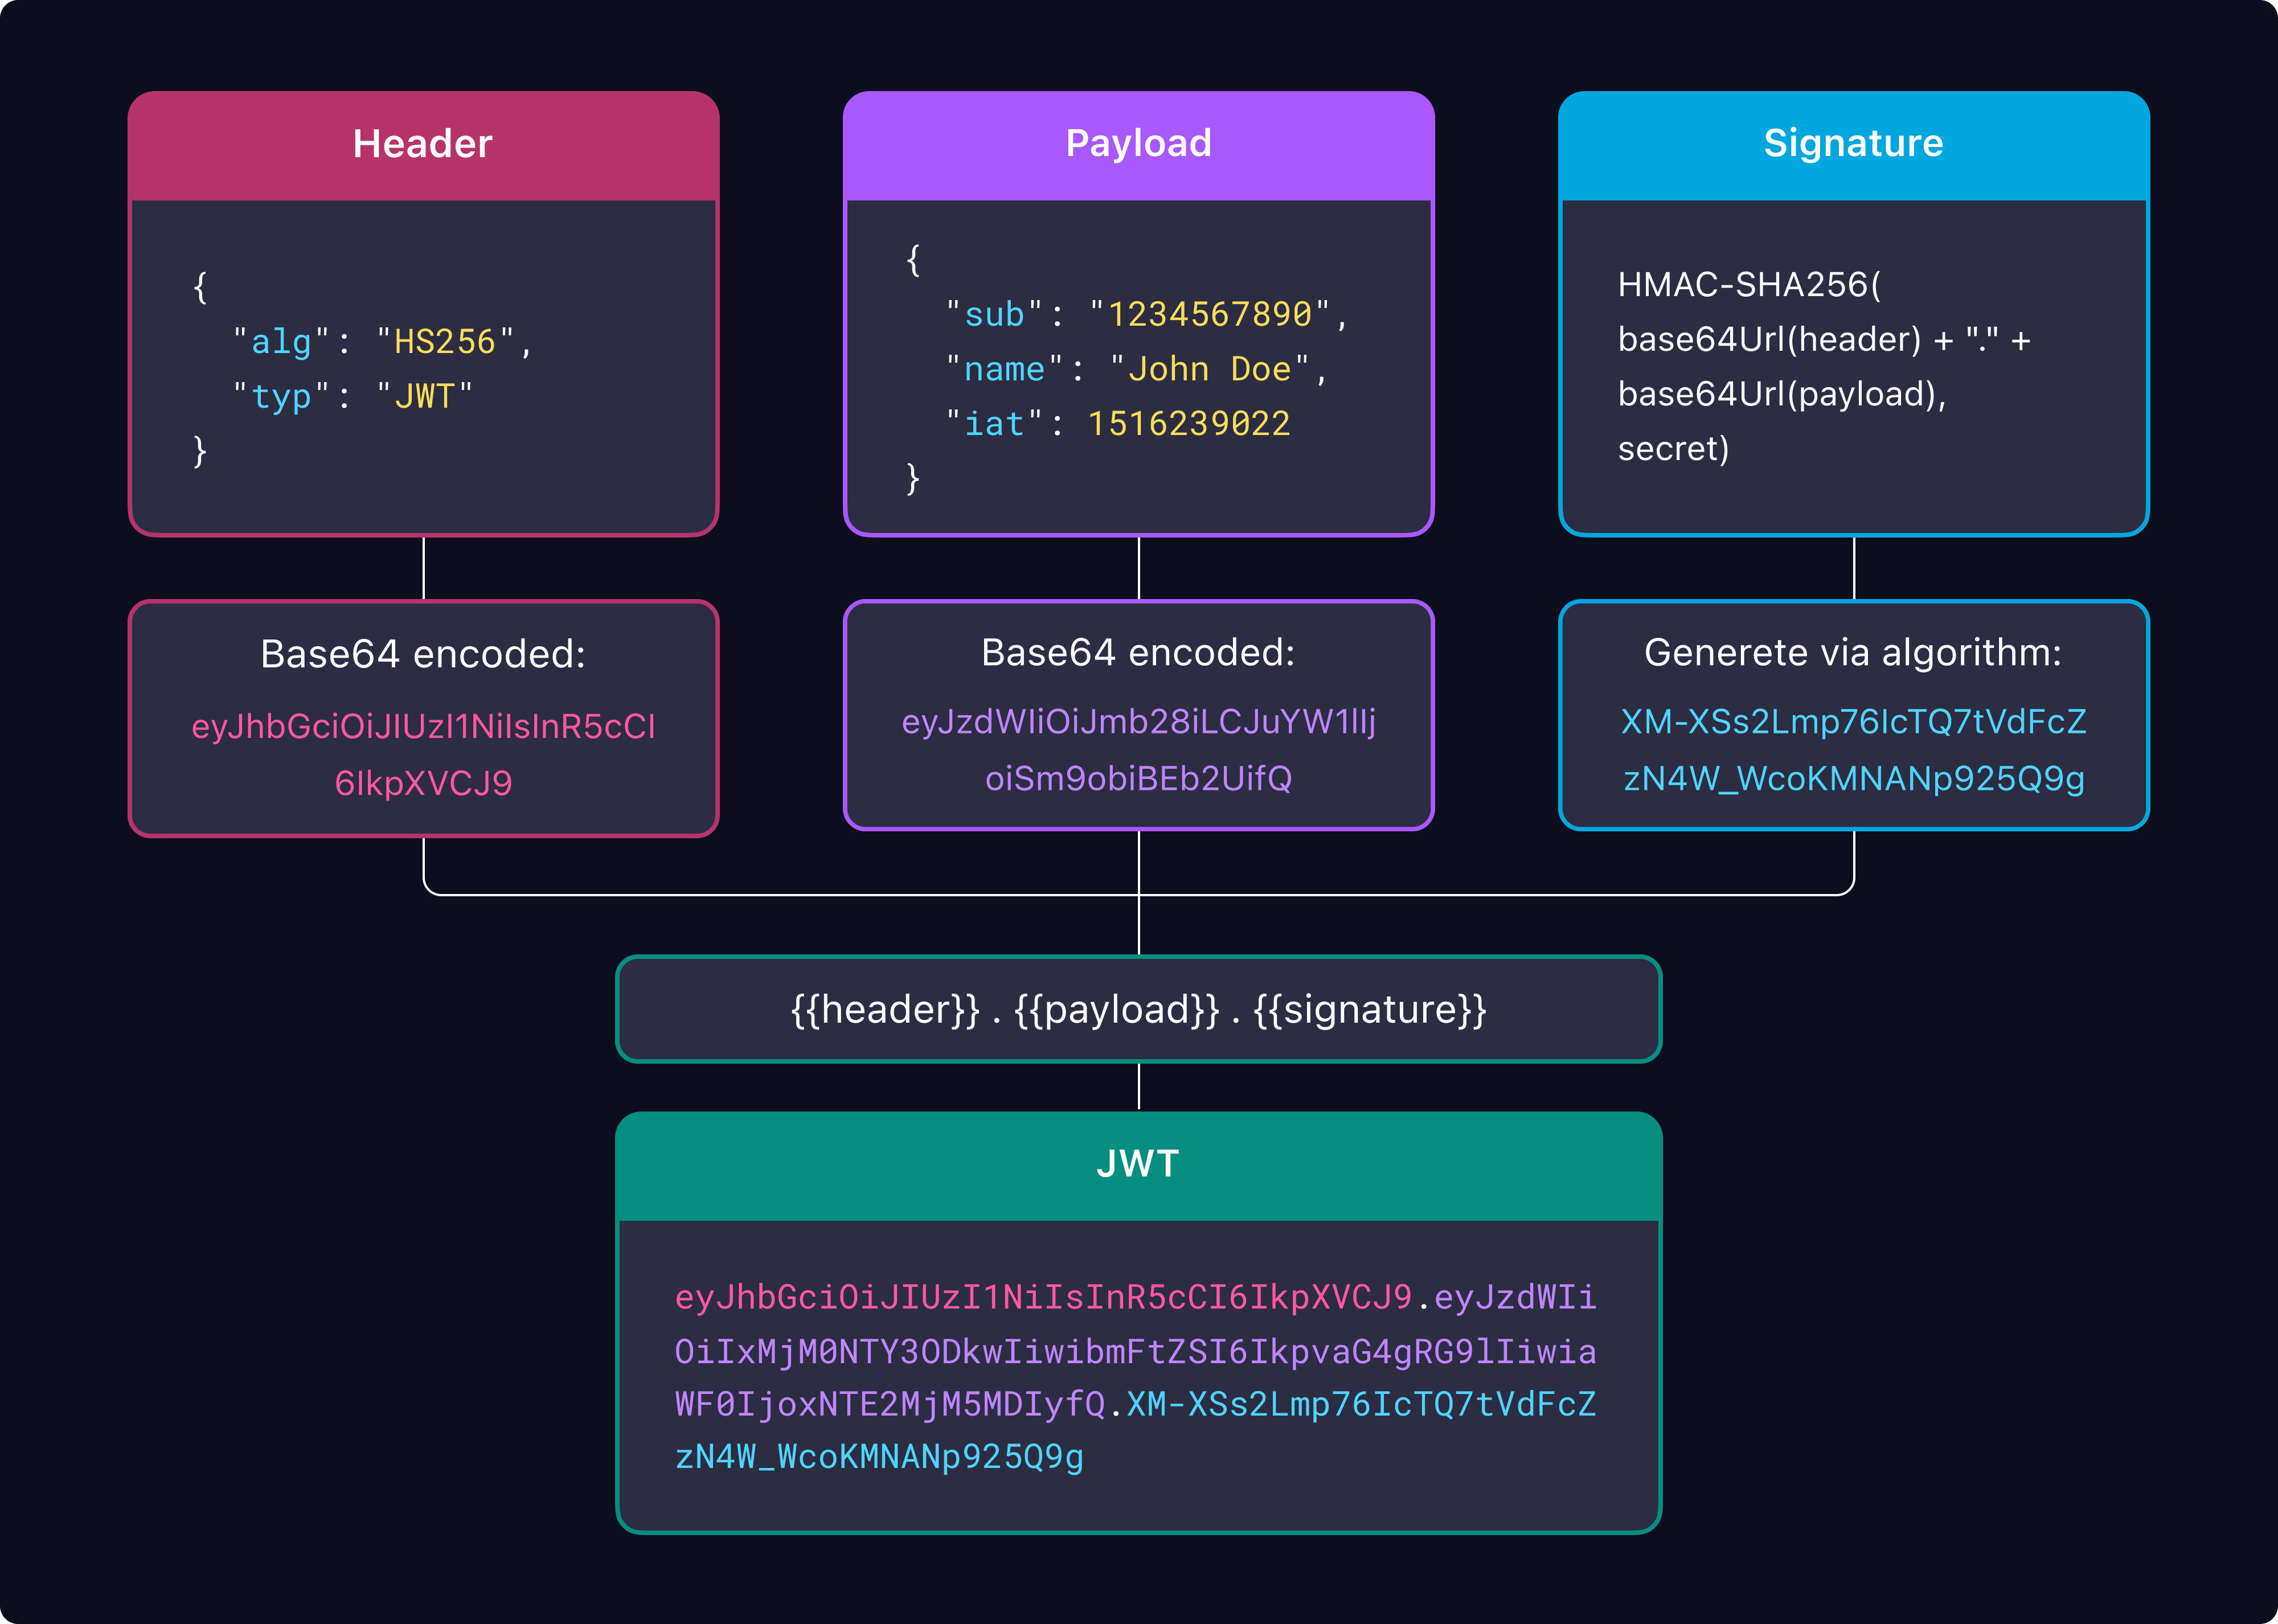
\includegraphics[width=0.9\textwidth,height=0.45\textheight,keepaspectratio]{assets/gambar/landasan-teori/jwt_structure.png}%
  }{%
    \framebox[\textwidth][c]{\rule{0pt}{3.5cm}\parbox{0.82\textwidth}{\centering \textbf{[Placeholder Diagram: Anatomi Struktur Tiga Segmen \textit{JSON Web Token} (JWT)]}\\\textit{Menampilkan segmen Header.Payload.Signature beserta struktur JSON klaim hasil dekode. (Menunggu berkas gambar)}}}}
  \caption{Anatomi Struktur Tiga Segmen \textit{JSON Web Token} (\texttt{Header.Payload.Signature})}
  \label{fig:teori_jwt}
\end{figure}

Berdasarkan Gambar~\ref{fig:teori_jwt}, segmen pertama adalah \textit{Header} yang memuat algoritma penandatanganan (seperti HS256 atau RS256) dan tipe token; segmen kedua adalah \textit{Payload} yang menyimpan daftar klaim identitas (\textit{registered claims} seperti \texttt{sub} dan \texttt{exp}, serta \textit{custom claims} seperti peran pengguna); dan segmen ketiga adalah \textit{Signature} hasil komputasi kriptografis untuk memverifikasi keutuhan isi token~\cite{rfc7519_jwt}. Mekanisme ini memungkinkan server layanan mikro memvalidasi identitas pengguna secara nir-status (\textit{stateless authentication}) tanpa bergantung pada memori sesi terpusat, meskipun memerlukan kebijakan masa berlaku pendek karena token yang belum kedaluwarsa tidak mudah dicabut secara sepihak.

%------------------------------------------------------------
\section{\textit{ROLE-BASED ACCESS CONTROL} (RBAC)}
%------------------------------------------------------------

\textbf{\textit{Role-Based Access Control}} (RBAC) sebagaimana distandarkan oleh NIST adalah model pengendalian akses otorisasi yang mengatur hak akses pengguna terhadap sumber daya sistem berdasarkan peran (\textit{roles}) yang ditugaskan kepada mereka dalam organisasi~\cite{ferraiolo2001rbac}. Berbeda dengan pendekatan tradisional yang menempelkan izin secara langsung ke akun individu, RBAC memperkenalkan lapisan abstraksi peran sehingga administrasi hak akses dapat dikelola secara terpusat dan konsisten sesuai prinsip hak akses minimal (\textit{least privilege}) serta pemisahan tugas (\textit{separation of duties}).

Model hubungan entitas inti pada standar RBAC NIST diilustrasikan pada Gambar~\ref{fig:teori_rbac}.

\begin{figure}[H]
  \centering
  \IfFileExists{assets/gambar/landasan-teori/rbac_model.png}{%
    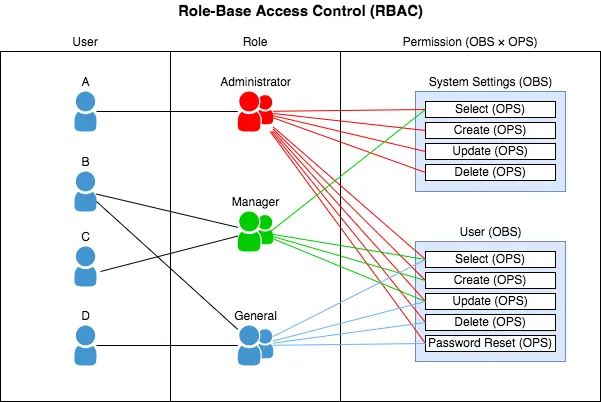
\includegraphics[width=0.88\textwidth,height=0.45\textheight,keepaspectratio]{assets/gambar/landasan-teori/rbac_model.png}%
  }{%
    \framebox[\textwidth][c]{\rule{0pt}{3.5cm}\parbox{0.82\textwidth}{\centering \textbf{[Placeholder Diagram: Model Hubungan Entitas Inti RBAC NIST]}\\\textit{Menampilkan relasi many-to-many antara Users, Roles, Permissions (Operations + Objects), dan Sessions. (Menunggu berkas gambar)}}}}
  \caption{Model Hubungan Entitas Inti \textit{Role-Based Access Control} (RBAC NIST)}
  \label{fig:teori_rbac}
\end{figure}

Mengacu pada Gambar~\ref{fig:teori_rbac}, setiap pengguna dapat memiliki satu atau lebih peran, dan setiap peran menghimpun sekumpulan izin operasi terhadap objek sumber daya tertentu~\cite{ferraiolo2001rbac}. Pada proyek MonGrid, model RBAC ini diperluas dengan skema otorisasi granular \textit{Employee Device Access} yang memvalidasi klaim JWT di sisi peladen (\texttt{DeviceAccessFilterService}) melalui penelusuran pohon hierarki aset ke bawah (\textit{downward tree traversal}) serta penegakan visibilitas di sisi antarmuka pengguna.

%------------------------------------------------------------
\section{\textit{LARGE LANGUAGE MODEL} (LLM)}
%------------------------------------------------------------

\textbf{\textit{Large Language Model}} (LLM) adalah model bahasa generatif berskala besar berbasis arsitektur \textbf{\textit{Transformer}} yang mengandalkan mekanisme \textit{self-attention} untuk memodelkan hubungan kontekstual antartoken dalam urutan teks panjang secara paralel~\cite{vaswani2017attention}. Dilatih pada korpus teks masif dengan miliaran parameter, LLM mampu memahami instruksi bahasa alami (\textit{instruction following}), melakukan penalaran kontekstual di dalam jendela konteks (\textit{in-context learning}), dan menyusun keluaran dalam format terstruktur.

Meskipun memiliki kapabilitas generalisasi bahasa yang luas, LLM standar memiliki tiga keterbatasan fundamental: (1) pengetahuan parametriknya bersifat statis dan membeku pada batas waktu pelatihan (\textit{knowledge cutoff}); (2) ukuran jendela konteks (\textit{context window}) membatasi volume informasi yang dapat diproses sekaligus; serta (3) dalam mode pemanggilan tunggal yang pasif, LLM rentan menghasilkan informasi keliru yang terdengar meyakinkan (\textit{hallucination}) ketika ditanya mengenai data operasional mutakhir. Keterbatasan inilah yang melatarbelakangi perlunya perluasan menuju sistem agen cerdas dan pemanggilan perkakas eksternal.

%------------------------------------------------------------
\section{\textit{VISION LANGUAGE MODEL} (VLM)}
%------------------------------------------------------------

\textbf{\textit{Vision Language Model}} (VLM) memperluas kapabilitas LLM ke ranah multimodal dengan memadukan penyandi visual (\textit{vision encoder}) dan lapisan proyektor penyelarasan (\textit{projection layer}) ke dalam ruang representasi model bahasa~\cite{liu2023visual}. Melalui arsitektur terpadu ini, model mampu memproses masukan citra digital dan instruksi teks secara bersamaan dalam satu lintasan pemahaman semantik.

Alur arsitektur konseptual VLM untuk ekstraksi dokumen multimodal ditunjukkan pada Gambar~\ref{fig:teori_vlm}.

\begin{figure}[H]
  \centering
  \IfFileExists{assets/gambar/landasan-teori/vlm_architecture.png}{%
    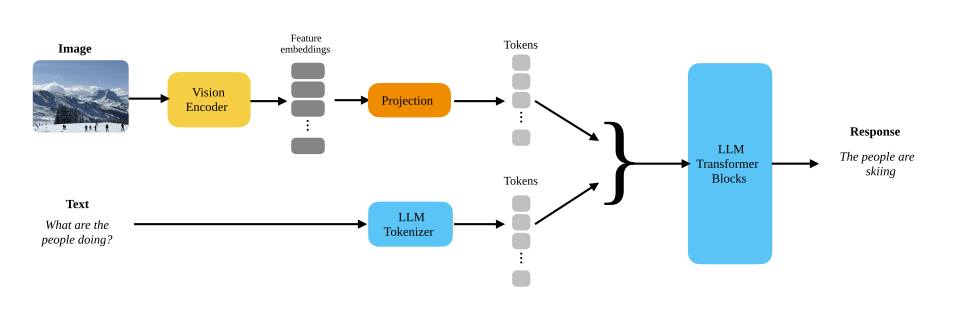
\includegraphics[width=0.9\textwidth,height=0.45\textheight,keepaspectratio]{assets/gambar/landasan-teori/vlm_architecture.png}%
  }{%
    \framebox[\textwidth][c]{\rule{0pt}{3.5cm}\parbox{0.82\textwidth}{\centering \textbf{[Placeholder Diagram: Alur Arsitektur Konseptual \textit{Vision Language Model} (VLM)]}\\\textit{Menampilkan Citra Dokumen $\rightarrow$ Vision Encoder $\rightarrow$ Projector digabung dengan Prompt Teks ke LLM Backbone. (Menunggu berkas gambar)}}}}
  \caption{Alur Arsitektur Konseptual \textit{Vision Language Model} (VLM) untuk Ekstraksi Dokumen Multimodal}
  \label{fig:teori_vlm}
\end{figure}

Berdasarkan Gambar~\ref{fig:teori_vlm}, representasi fitur visual dari dokumen dipetakan ke ruang semantik yang dapat dipahami oleh tulang punggung LLM sehingga model dapat langsung mengekstrak entitas bermakna ke dalam format JSON terstruktur~\cite{liu2023visual}. Dibandingkan perangkat lunak OCR konvensional berbasis templat koordinat kaku, VLM jauh lebih tangguh menghadapi variasi tata letak, kualitas foto lapangan, dan tulisan tangan. Pada proyek PT Makassar Trans, kapabilitas ini diterapkan melalui \textbf{Ollama Vision}~\cite{ollama_vision} untuk membaca dokumen tanda terima pengiriman barang menjadi draf terstruktur.

%------------------------------------------------------------
\section{\textit{AGENTIC AI}}
%------------------------------------------------------------

\textbf{\textit{Agentic AI}} adalah paradigma perancangan sistem kecerdasan buatan otonom yang menempatkan LLM sebagai inti pengambil keputusan (\textit{reasoning core}) di dalam sebuah sistem yang mampu merencanakan, mengingat konteks, menggunakan perkakas eksternal, dan berinteraksi secara iteratif dengan lingkungannya guna mencapai tujuan tertentu~\cite{wang2024survey}. Berbeda dari pola penggunaan LLM tradisional yang bersifat pasif satu putaran (\textit{single-turn prompt-response}), sistem berbasis agen memiliki otonomi untuk memecah tugas kompleks menjadi sub-langkah dan memverifikasi hasilnya sebelum menyimpulkan jawaban.

Arsitektur konseptual sistem \textit{Agentic AI} otonom terdiri atas empat komponen utama sebagaimana diilustrasikan pada Gambar~\ref{fig:teori_agentic_ai}.

\begin{figure}[H]
  \centering
  \IfFileExists{assets/gambar/landasan-teori/agentic_ai_architecture.png}{%
    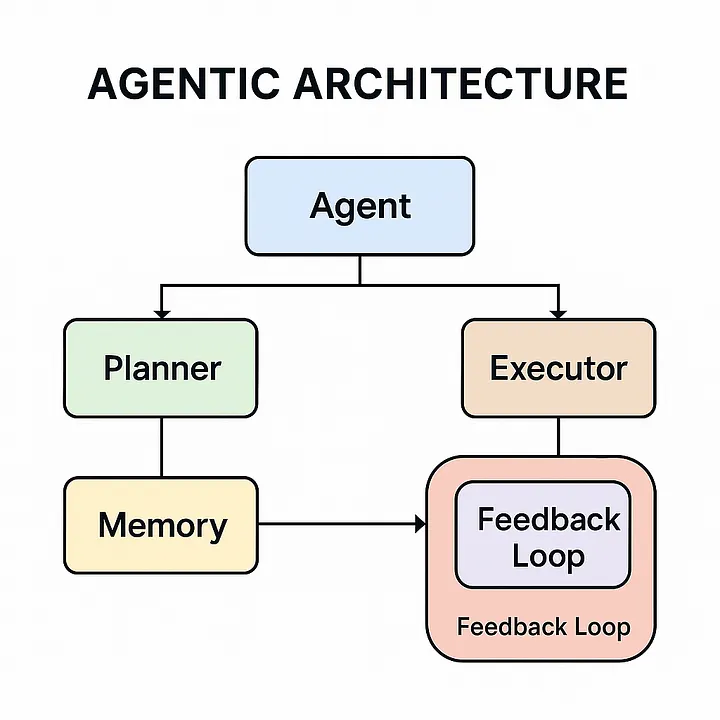
\includegraphics[width=0.88\textwidth,height=0.45\textheight,keepaspectratio]{assets/gambar/landasan-teori/agentic_ai_architecture.png}%
  }{%
    \framebox[\textwidth][c]{\rule{0pt}{3.5cm}\parbox{0.82\textwidth}{\centering \textbf{[Placeholder Diagram: Arsitektur Komponen Utama Sistem \textit{Agentic AI} Otonom]}\\\textit{Menampilkan LLM Core terhubung dengan pilar Planning, Memory/State, Tools/Action, dan Environment Loop. (Menunggu berkas gambar)}}}}
  \caption{Arsitektur Komponen Utama Sistem \textit{Agentic AI} Otonom}
  \label{fig:teori_agentic_ai}
\end{figure}

Mengacu pada Gambar~\ref{fig:teori_agentic_ai}, keempat pilar tersebut mencakup modul perencanaan (\textit{planning}) untuk menyusun strategi, modul memori (\textit{memory}) untuk menyimpan status jangka pendek maupun pengetahuan jangka panjang, modul perkakas (\textit{tool use}) untuk bertindak di dunia nyata, serta siklus umpan balik lingkungan (\textit{observation})~\cite{wang2024survey}. Ketika beberapa agen dengan spesialisasi peran berbeda dikoordinasikan bersama, paradigma ini berkembang menjadi orkestrasi multi-agen. Paradigma \textit{Agentic AI} menjadi landasan konseptual bagi modul *AI Chat* otonom pada MonGrid dan keseluruhan ekosistem Nedo Agentic Platform.

%------------------------------------------------------------
\section{\textit{TOOL CALLING} (PEMANGGILAN PERKAKAS)}
%------------------------------------------------------------

\textbf{\textit{Tool Calling}} (sering disebut juga \textit{Function Calling}) adalah mekanisme antarmuka terstruktur yang memungkinkan model bahasa memilih dan memanggil fungsi, kueri basis data, atau API eksternal secara deterministik berdasarkan skema deskripsi yang disediakan oleh aplikasi induk~\cite{schick2023toolformer}. Melalui kapabilitas ini, model tidak lagi dipaksa menebak fakta operasional dari memori parametriknya, melainkan mendelegasikan pengambilan data maupun eksekusi aksi nyata ke perkakas yang tepat.

Siklus pertukaran pesan dalam mekanisme \textit{Tool Calling} antara aplikasi orkestrator, LLM, dan fungsi eksternal ditunjukkan pada Gambar~\ref{fig:teori_tool_calling}.

\begin{figure}[H]
  \centering
  \IfFileExists{assets/gambar/landasan-teori/tool_calling_sequence.png}{%
    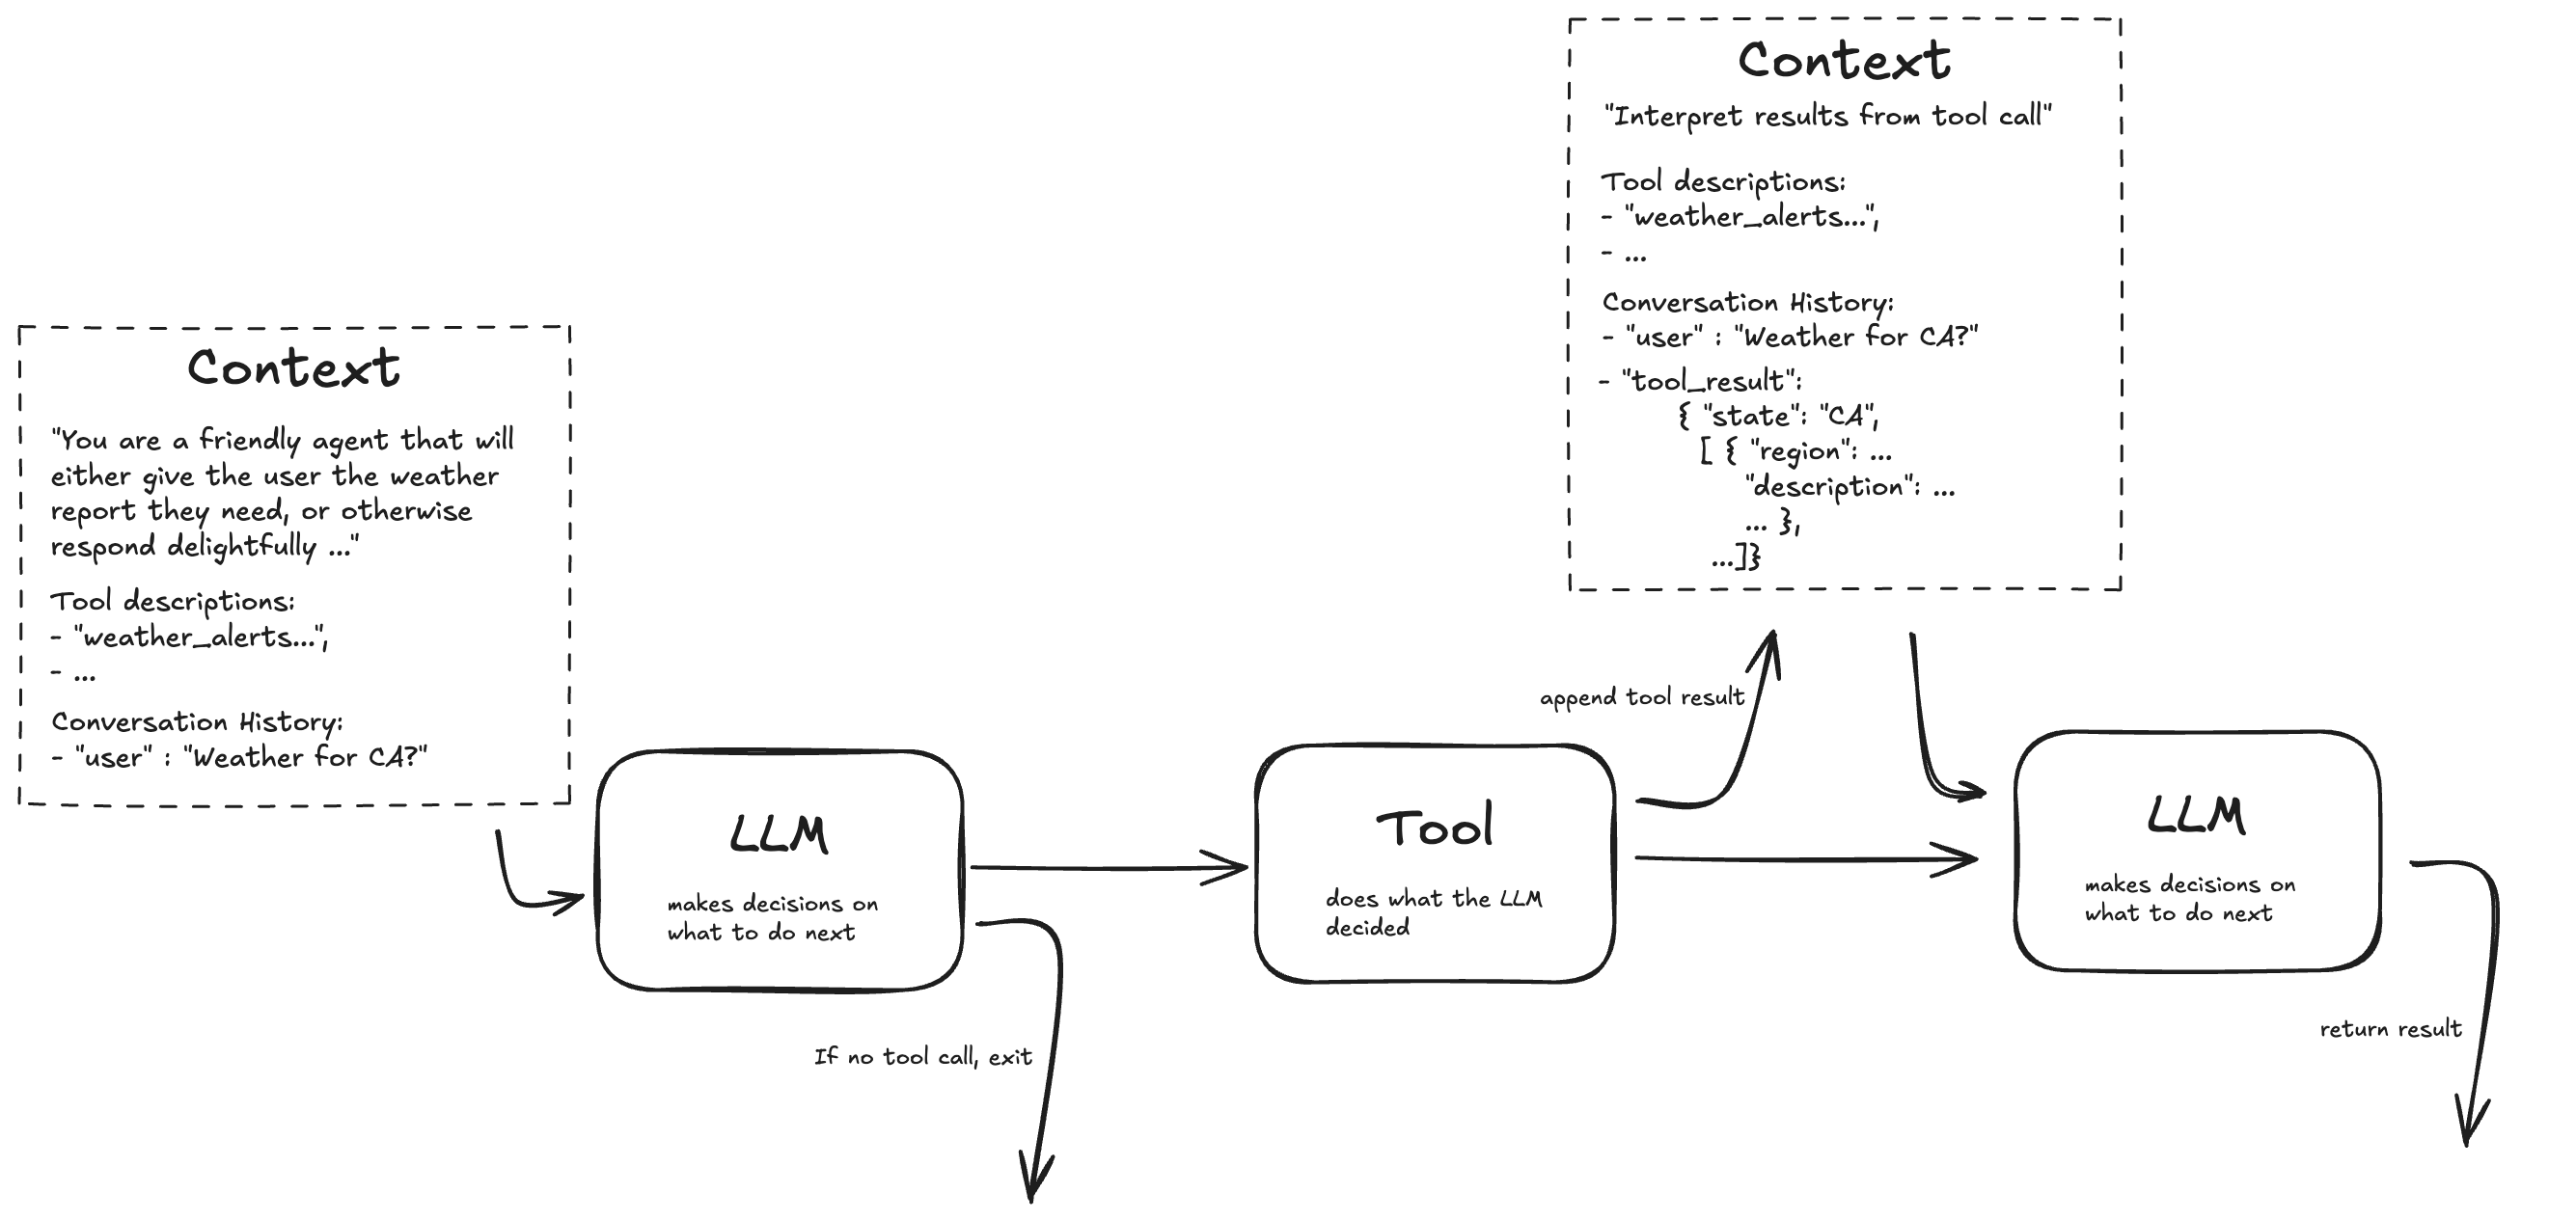
\includegraphics[width=0.9\textwidth,height=0.45\textheight,keepaspectratio]{assets/gambar/landasan-teori/tool_calling_sequence.png}%
  }{%
    \framebox[\textwidth][c]{\rule{0pt}{3.5cm}\parbox{0.82\textwidth}{\centering \textbf{[Placeholder Diagram: Diagram Urutan Siklus Mekanisme \textit{Tool Calling}]}\\\textit{Menampilkan pertukaran Prompt + Schema $\rightarrow$ JSON tool\_call $\rightarrow$ Eksekusi Fungsi $\rightarrow$ tool\_result $\rightarrow$ Jawaban Akhir. (Menunggu berkas gambar)}}}}
  \caption{Diagram Urutan Siklus Mekanisme \textit{Tool Calling} pada Model Bahasa}
  \label{fig:teori_tool_calling}
\end{figure}

Sebagaimana terlihat pada Gambar~\ref{fig:teori_tool_calling}, aplikasi mengirimkan instruksi pengguna beserta daftar skema JSON definisi perkakas; apabila membutuhkan data eksternal, LLM mengembalikan objek terstruktur berisi nama fungsi dan argumennya (\texttt{tool\_call}); aplikasi kemudian mengeksekusi fungsi tersebut dan menyuntikkan hasilnya (\texttt{tool\_result}) kembali ke konteks LLM untuk menyusun jawaban akhir. Mekanisme ini mendasari perombakan *AI Chat* MonGrid dari penyuntikan konteks statis menjadi pemanggilan instrumen dinamis (\texttt{Nedo.AspNet.AgentOrchestration}) serta taksonomi perkakas 4-tier pada Nedo Agentic Platform.

%------------------------------------------------------------
\section{POLA PENALARAN DAN TINDAKAN (\textit{REACT})}
%------------------------------------------------------------

\textbf{ReAct} (\textit{Reasoning and Acting}) adalah paradigma kendali eksekusi agen cerdas yang menginterleavasi jejak penalaran verbal (\textit{Thought}), eksekusi tindakan melalui pemanggilan perkakas (\textit{Action}), dan pembacaan umpan balik hasil dari lingkungan (\textit{Observation}) secara berulang dalam satu siklus tertutup hingga tujuan tercapai~\cite{yao2023react}. Pendekatan ini menggabungkan kekuatan penalaran langkah-demi-langkah dengan interaksi dunia nyata secara bersamaan.

Siklus perulangan pada pola penalaran dan tindakan ReAct ditunjukkan pada Gambar~\ref{fig:teori_react}.

\begin{figure}[H]
  \centering
  \IfFileExists{assets/gambar/landasan-teori/react_loop.png}{%
    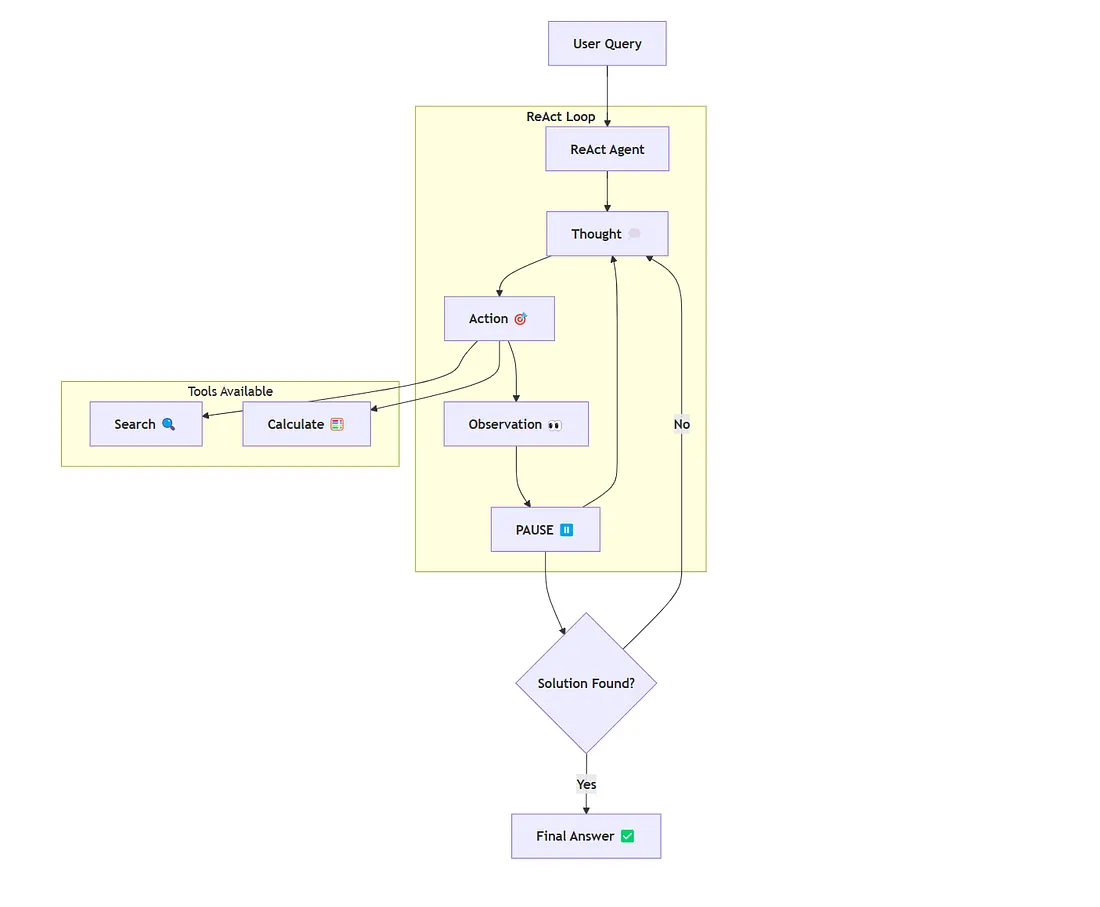
\includegraphics[width=0.88\textwidth,height=0.45\textheight,keepaspectratio]{assets/gambar/landasan-teori/react_loop.png}%
  }{%
    \framebox[\textwidth][c]{\rule{0pt}{3.5cm}\parbox{0.82\textwidth}{\centering \textbf{[Placeholder Diagram: Siklus Perulangan \textit{Thought--Action--Observation} Pola ReAct]}\\\textit{Menampilkan loop tertutup Thought $\rightarrow$ Action $\rightarrow$ Observation berulang hingga Final Answer. (Menunggu berkas gambar)}}}}
  \caption{Siklus Perulangan \textit{Thought--Action--Observation} pada Pola \textit{ReAct}}
  \label{fig:teori_react}
\end{figure}

Berdasarkan Gambar~\ref{fig:teori_react}, berbeda dari metode \textit{Chain-of-Thought} (CoT) murni yang hanya menalar secara internal tanpa verifikasi eksternal, setiap langkah \textit{Observation} pada ReAct membumikan penalaran agen terhadap fakta aktual dan memungkinkan koreksi rencana secara dinamis saat terjadi galat~\cite{yao2023react}. Pola ini menjadi inti dari mesin eksekusi \textit{In-House Native ReAct Engine} (\texttt{nedo.runner.engine}) pada Nedo Agentic Platform (lengkap dengan mekanisme \textit{Adaptive Cognitive Pacing}) serta siklus perulangan agen pada *AI Chat* MonGrid.

%------------------------------------------------------------
\section{\textit{MODEL CONTEXT PROTOCOL} (MCP)}
%------------------------------------------------------------

\textbf{\textit{Model Context Protocol}} (MCP) adalah standar protokol terbuka berbasis **JSON-RPC 2.0** yang dirancang untuk menstandarkan cara aplikasi AI dan agen cerdas terhubung dengan sumber data maupun perkakas eksternal secara modular~\cite{mcp_spec}. Sebelum adanya standar ini, setiap aplikasi agen harus membangun konektor khusus untuk tiap sumber data (masalah integrasi $N \times M$); MCP menyederhanakannya menjadi pola antarmuka tunggal ($N + M$) yang dapat digunakan ulang lintas platform.

Arsitektur komunikasi antarperan dalam spesifikasi \textit{Model Context Protocol} diperlihatkan pada Gambar~\ref{fig:teori_mcp}.

\begin{figure}[H]
  \centering
  \IfFileExists{assets/gambar/landasan-teori/mcp_architecture.png}{%
    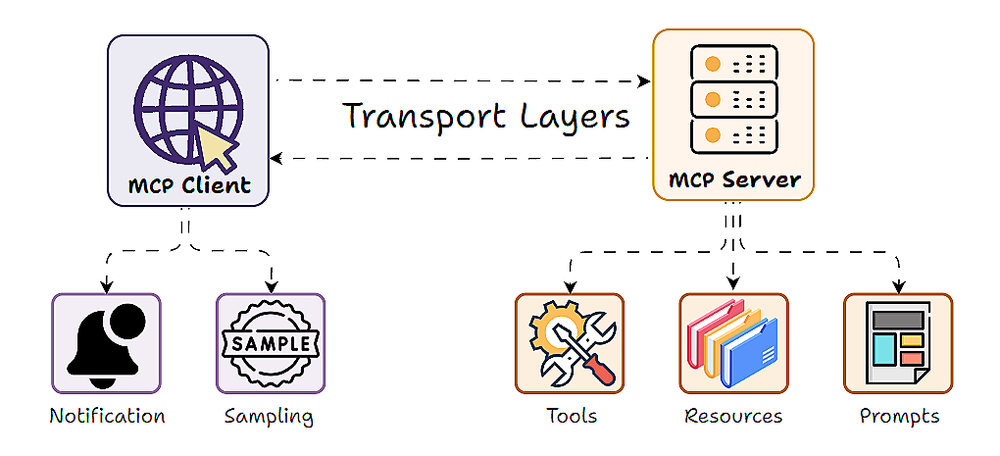
\includegraphics[width=0.9\textwidth,height=0.45\textheight,keepaspectratio]{assets/gambar/landasan-teori/mcp_architecture.png}%
  }{%
    \framebox[\textwidth][c]{\rule{0pt}{3.5cm}\parbox{0.82\textwidth}{\centering \textbf{[Placeholder Diagram: Arsitektur Komunikasi \textit{Host--Client--Server} MCP]}\\\textit{Menampilkan MCP Host/Client berkomunikasi via JSON-RPC 2.0 dengan banyak MCP Server (Tools, Resources, Prompts). (Menunggu berkas gambar)}}}}
  \caption{Arsitektur Komunikasi \textit{Host--Client--Server} pada \textit{Model Context Protocol} (MCP)}
  \label{fig:teori_mcp}
\end{figure}

Mengacu pada Gambar~\ref{fig:teori_mcp}, arsitektur MCP membagi komponen menjadi \textit{MCP Host} (aplikasi agen induk yang mengelola satu atau lebih \textit{MCP Client}) dan \textit{MCP Server} (layanan terpisah yang mengekspos kapabilitas berupa \textit{Tools}, \textit{Resources}, dan \textit{Prompts}) melalui transport \textit{stdio} lokal maupun HTTP/\textit{Streamable SSE} jarak jauh~\cite{mcp_spec}. Pada Nedo Agentic Platform, protokol ini diimplementasikan menggunakan pustaka FastMCP untuk layanan mikro internal (\texttt{nedo-browser-mcp}, \texttt{nedo-web-extract-mcp}, dan \texttt{kali-mcp}) maupun integrasi layanan eksternal per ruang kerja.

%------------------------------------------------------------
\section{\textit{CONTAINER SANDBOXING}}
%------------------------------------------------------------

\textbf{\textit{Container Sandboxing}} dalam konteks keamanan sistem informasi dan agen otonom adalah teknik pengisolasian lingkungan eksekusi untuk menjalankan kode pemrograman maupun perintah terminal yang dihasilkan secara dinamis oleh LLM (kode tak tepercaya / \textit{untrusted code}) tanpa membahayakan sistem operasi induk~\cite{souppaya2017nist}. Isolasi di level kontainer bertumpu pada dua mekanisme inti kernel Linux: \textit{Namespaces} untuk memisahkan ruang pandang proses (PID), antarmuka jaringan, serta sistem berkas dari host, dan \textit{Control Groups} (\textit{cgroups}) untuk membatasi kuota CPU serta penggunaan RAM secara ketat~\cite{souppaya2017nist, docker_doc}.

Untuk meminimalisir permukaan serangan dan mencegah persistensi jejak berbahaya antartugas, sistem agen menerapkan pola kontainer sementara (\textit{ephemeral container}), di mana kontainer dibuat khusus untuk satu sesi eksekusi dengan akses jaringan diputus (\texttt{--network none}), batas waktu eksekusi ketat, dan langsung dihancurkan setelah hasil dikembalikan. Mekanisme ini diterapkan pada perkakas Tier 2 Nedo Agentic Platform untuk mengeksekusi kode Python maupun perintah terminal yang dihasilkan oleh agen secara terisolasi.

%------------------------------------------------------------
\section{\textit{DIRECTED ACYCLIC GRAPH} (DAG)}
%------------------------------------------------------------

\textbf{\textit{Directed Acyclic Graph}} (DAG) dalam teori graf dan algoritma adalah graf berarah $G = (V, E)$ yang tidak mengandung lintasan siklus tertutup (\textit{cycle-free}), artinya tidak ada simpul yang dapat kembali ke dirinya sendiri dengan mengikuti arah sisi (\textit{directed edges})~\cite{cormen2022introduction}. Properti bebas siklus ini menjamin bahwa setiap DAG memiliki sekurang-kurangnya satu urutan linier yang konsisten terhadap arah ketergantungannya melalui algoritma pengurutan topologis (\textit{topological sorting})~\cite{cormen2022introduction}.

Dalam perancangan sistem orkestrasi alur kerja terdistribusi, setiap simpul ($V$) merepresentasikan unit pekerjaan dan setiap sisi berarah ($E$) menyatakan relasi prasyarat antara tugas pendahulu (\textit{predecessor}) dan tugas penerus (\textit{successor}), sebagaimana ditunjukkan pada Gambar~\ref{fig:teori_dag}.

\begin{figure}[H]
  \centering
  \IfFileExists{assets/gambar/landasan-teori/dag_workflow.png}{%
    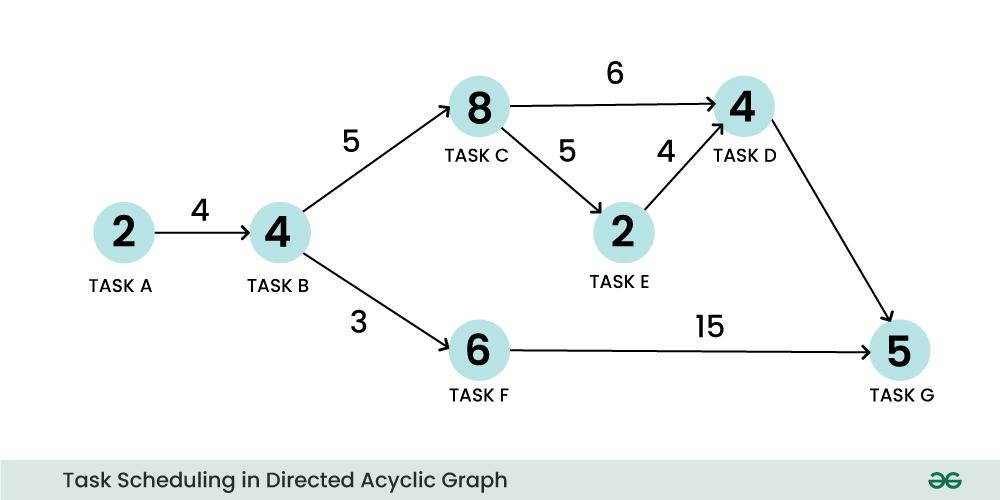
\includegraphics[width=0.88\textwidth,height=0.45\textheight,keepaspectratio]{assets/gambar/landasan-teori/dag_workflow.png}%
  }{%
    \framebox[\textwidth][c]{\rule{0pt}{3.5cm}\parbox{0.82\textwidth}{\centering \textbf{[Placeholder Diagram: Representasi Graf Ketergantungan Tugas \textit{Directed Acyclic Graph} (DAG)]}\\\textit{Menampilkan simpul tugas berarah tanpa siklus dengan cabang eksekusi paralel dan titik penggabungan. (Menunggu berkas gambar)}}}}
  \caption{Representasi Graf Ketergantungan Tugas \textit{Directed Acyclic Graph} (DAG)}
  \label{fig:teori_dag}
\end{figure}

Berdasarkan Gambar~\ref{fig:teori_dag}, struktur DAG memungkinkan mesin orkestrasi mengidentifikasi cabang tugas yang tidak saling bergantung untuk dieksekusi secara paralel sekaligus mencegah kondisi kebuntuan siklus (\textit{deadlock}). Pada Nedo Agentic Platform, model DAG digunakan oleh pekerja Celery untuk mengorkestrasi tugas multi-agen, menegakkan aturan penulisan berkas bebas tabrakan (\textit{Single-Writer Guardrail}), serta divisualisasikan pada antarmuka \textit{Run Board DAG}.

%------------------------------------------------------------
\section{\textit{HUMAN-IN-THE-LOOP} (HITL)}
%------------------------------------------------------------

\textbf{\textit{Human-in-the-Loop}} (HITL) adalah paradigma perancangan sistem kecerdasan buatan dan otomasi alur kerja yang mengintegrasikan keterlibatan, penilaian, serta persetujuan operator manusia secara terstruktur pada titik-titik kritis di dalam siklus eksekusi mesin~\cite{mosqueira2023human}. Alih-alih memberikan otonomi mutlak tanpa pengawasan yang berisiko memicu tindakan merusak atau kesalahan interpretasi ketika menghadapi instruksi ambigu, HITL menempatkan manusia sebagai pengendali akhir (\textit{oversight gate}) maupun sumber klarifikasi kontekstual.

Pada sistem agen otonom terdistribusi, interaksi HITL umumnya diwujudkan melalui pola \textit{interrupt--freeze--resume} sebagaimana diilustrasikan pada Gambar~\ref{fig:teori_hitl}.

\begin{figure}[H]
  \centering
  \IfFileExists{assets/gambar/landasan-teori/hitl_workflow.png}{%
    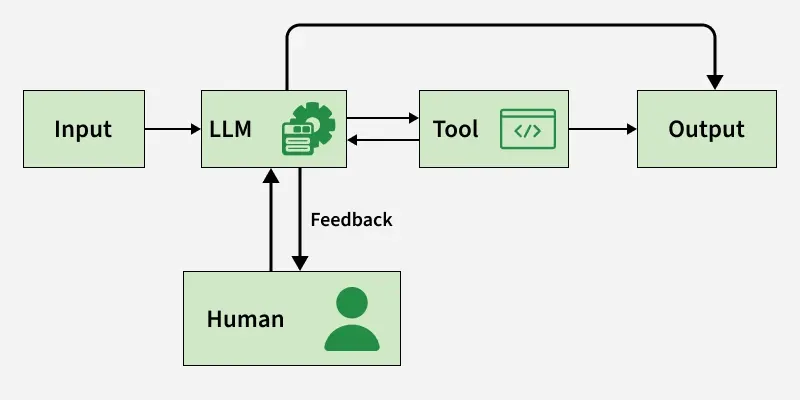
\includegraphics[width=0.9\textwidth,height=0.45\textheight,keepaspectratio]{assets/gambar/landasan-teori/hitl_workflow.png}%
  }{%
    \framebox[\textwidth][c]{\rule{0pt}{3.5cm}\parbox{0.82\textwidth}{\centering \textbf{[Placeholder Diagram: Alur Mekanisme \textit{Interrupt--Approval--Resume} pada \textit{Human-in-the-Loop}]}\\\textit{Menampilkan eksekusi berhenti sementara, masuk antrean operator, lalu lanjut setelah persetujuan/masukan diberikan. (Menunggu berkas gambar)}}}}
  \caption{Alur Mekanisme \textit{Interrupt--Approval--Resume} pada Siklus \textit{Human-in-the-Loop} (HITL)}
  \label{fig:teori_hitl}
\end{figure}

Mengacu pada Gambar~\ref{fig:teori_hitl}, ketika agen memerlukan klarifikasi atau menyentuh kebijakan otorisasi perkakas berisiko, status eksekusi dibekukan secara aman di penyimpanan persisten sembari menjeda batas waktu eksekusi, dan tugas dialihkan ke antrean perhatian operator~\cite{mosqueira2023human}. Setelah operator memberikan masukan atau persetujuan, mesin melanjutkan siklus tepat dari titik pemberhentian sebelumnya. Pada proyek kerja praktik, HITL diterapkan secara berlapis pada Nedo Agentic Platform (\texttt{ask\_requester}, kebijakan \textit{Needs approval}, antrean \textit{Needs you}, dan konfirmasi pembuatan PDF) serta secara operasional melalui verifikasi petugas atas draf OCR VLM pada PT Makassar Trans.

%------------------------------------------------------------
\section{REACT}
%------------------------------------------------------------

\textbf{React} adalah pustaka JavaScript deklaratif berbasis komponen yang dikembangkan untuk membangun antarmuka pengguna web interaktif maupun aplikasi satu halaman (\textit{Single-Page Application} / SPA)~\cite{react_doc}. Alih-alih memanipulasi pohon dokumen peramban (\textit{Real DOM}) secara imperatif yang mahal secara komputasi, React memelihara representasi memori ringan bernama \textit{Virtual DOM}, menghitung selisih perubahan antarstatus melalui proses rekonsiliasi, dan hanya menerapkan pembaruan minimal yang diperlukan ke antarmuka peramban~\cite{react_doc}.

Dengan dukungan aliran data searah (\textit{unidirectional data flow}) dan antarmuka fungsional \textit{React Hooks} untuk mengelola status lokal serta efek samping komponen, kode antarmuka menjadi lebih modular dan mudah diprediksi. Pada proyek MonGrid dan Nedo Agentic Platform, React 19 dipadukan dengan \textbf{TypeScript} untuk keamanan tipe data statis, \textbf{Vite} sebagai perkakas kompilasi cepat berbasis modul ES, serta \textbf{Tailwind CSS} untuk penataan gaya antarmuka yang konsisten.

%------------------------------------------------------------
\section{TANSTACK QUERY}
%------------------------------------------------------------

Dalam pengembangan aplikasi web modern, terdapat perbedaan mendasar antara \textit{client state} (status antarmuka lokal yang sepenuhnya dikuasai peramban seperti modal atau tab aktif) dan \textit{server state} (data jarak jauh yang tersimpan di server, bersifat asinkron, dan rentan usang ketika berubah oleh pihak lain)~\cite{tanstack_query}. \textbf{TanStack Query} (sebelumnya dikenal sebagai React Query) adalah pustaka manajemen status asinkron yang dirancang khusus untuk mengambil, menyimpan di tembolok (\textit{caching}), menyinkronkan, dan memutakhirkan \textit{server state} di sisi klien~\cite{tanstack_query}.

TanStack Query mengorganisasikan data tembolok menggunakan pengenal unik berbasis larik (\textit{query keys}), mengelola siklus hidup kesegaran data (\textit{fresh}, \textit{stale}, \textit{fetching}), melakukan deduplikasi permintaan jaringan yang identik secara otomatis, serta menyediakan antarmuka manipulasi tembolok langsung di memori (\texttt{setQueryData})~\cite{tanstack_query}. Pada arsitektur \textit{dual-channel} MonGrid, mekanisme \texttt{setQueryData} dimanfaatkan untuk melakukan \textit{in-memory cache patching} langsung dari pesan STOMP WebSocket tanpa memicu permintaan ulang HTTP yang boros.

%------------------------------------------------------------
\section{GOOGLE MAPS JAVASCRIPT API}
%------------------------------------------------------------

Sistem Informasi Geografis (\textit{Geographic Information System} / GIS) berbasis web memungkinkan penyajian, analisis, dan interaksi data spasial secara langsung melalui peramban web. \textbf{Google Maps JavaScript API} adalah antarmuka pemrograman resmi dari Google Maps Platform yang menyediakan kanvas peta digital interaktif beserta lapisan kontrol spasial di sisi klien~\cite{google_maps_js}.

Secara teknis, API ini memetakan titik koordinat geografis lintang dan bujur (\textit{latitude/longitude}) ke dalam sistem proyeksi peta \textit{Web Mercator} dengan dukungan berbagai tingkat pembesaran (\textit{zoom level}), kustomisasi gaya peta, pemasangan penanda khusus (\textit{custom markers}), pengelompokan penanda otomatis pada kepadatan tinggi (\textit{marker clustering}), serta jendela informasi interaktif (\textit{info window})~\cite{google_maps_js}. Pada proyek MonGrid, API ini mendasari modul \textit{GIS Map View} untuk memvisualisasikan sebaran lokasi gardu, gedung, transformator, dan indikator status alarm jaringan listrik secara waktu nyata.

%------------------------------------------------------------
\section{THREE.JS}
%------------------------------------------------------------

\textbf{Three.js} adalah pustaka grafis 3D sumber terbuka lintas peramban yang membungkus kompleksitas antarmuka pemrograman grafis tingkat rendah **WebGL** (*Web Graphics Library*)—yang memanfaatkan akselerasi perangkat keras GPU langsung di dalam elemen kanvas HTML—menjadi abstraksi pemrograman berorientasi objek yang lebih ringkas~\cite{threejs_doc}. Melalui abstraksi tersebut, pengembang dapat merender adegan 3D interaktif di peramban tanpa harus menulis kode \textit{shader} GLSL maupun manajemen penyangga WebGL secara manual dari awal.

Pengorganisasian elemen visual 3D pada Three.js disusun menggunakan struktur hierarki pohon bernama \textit{Scene Graph} yang menghubungkan \textit{Renderer}, \textit{Scene}, \textit{Camera}, sumber pencahayaan (\textit{Lights}), dan objek \textit{Mesh} (gabungan \textit{Geometry} dan \textit{Material})~\cite{threejs_doc}. Pada Nedo Agentic Platform, Three.js melalui ekosistem React Three Fiber digunakan untuk membangun antarmuka spasial \textit{Live Virtual Office} dalam mode denah 2D, isometrik 3D, dan navigasi sudut pandang langsung. Struktur hierarki \textit{Scene Graph} Three.js ditunjukkan pada Gambar~\ref{fig:teori_threejs}.

\begin{figure}[H]
  \centering
  \IfFileExists{assets/gambar/landasan-teori/threejs_scene_graph.png}{%
    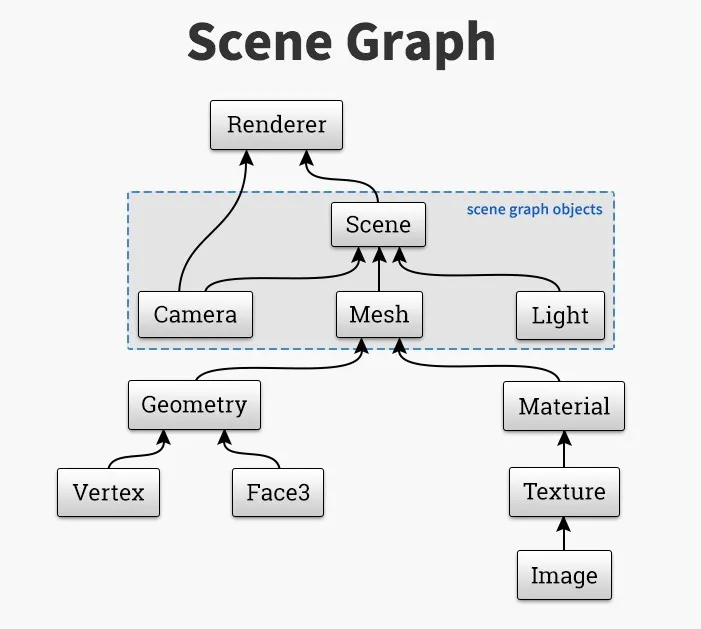
\includegraphics[width=0.88\textwidth,height=0.45\textheight,keepaspectratio]{assets/gambar/landasan-teori/threejs_scene_graph.png}%
  }{%
    \framebox[\textwidth][c]{\rule{0pt}{3.5cm}\parbox{0.82\textwidth}{\centering \textbf{[Placeholder Gambar: Hierarki Struktur \textit{Scene Graph} pada Three.js]}\\\textit{Menunggu berkas gambar/diagram resmi dokumentasi Three.js.}}}}
  \caption{Hierarki Struktur \textit{Scene Graph} pada Three.js}
  \label{fig:teori_threejs}
\end{figure}

Mengacu pada Gambar~\ref{fig:teori_threejs}, komponen \textit{Renderer} berada di puncak hierarki untuk merender adegan berdasarkan sudut pandang \textit{Camera} dan isi \textit{Scene}. Di dalam \textit{Scene} terkumpul objek-objek \textit{scene graph} mencakup \textit{Camera}, \textit{Light}, dan \textit{Mesh}, di mana setiap \textit{Mesh} dibangun dari perpaduan \textit{Geometry} (tersusun atas \textit{Vertex} dan \textit{Face3}) serta \textit{Material} (yang dapat memuat \textit{Texture} dari sumber \textit{Image}).

%------------------------------------------------------------
\section{FLUTTER}
%------------------------------------------------------------

\textbf{Flutter} adalah kerangka kerja pengembangan aplikasi lintas platform (\textit{Software Development Kit} / SDK) yang memungkinkan kompilasi satu basis kode berbahasa Dart secara \textit{ahead-of-time} (AOT) menjadi kode mesin natif untuk sistem operasi Android maupun iOS~\cite{flutter_architecture}. Berbeda dari kerangka kerja hibrida yang membungkus komponen antarmuka bawaan sistem operasi (\textit{OEM widgets}) melalui jembatan JavaScript, Flutter menyusun seluruh tampilan dari pohon \textit{Widget} komposisional dan menggambar setiap pikselnya secara mandiri ke kanvas menggunakan mesin grafis berkinerja tinggi (Skia/Impeller).

Dalam panduan arsitektur resminya, Flutter menganjurkan pemisahan tanggung jawab ke dalam lapisan \textit{UI/Presentation}, \textit{Domain}, dan \textit{Data} agar kode aplikasi petugas lapangan pada proyek PT Makassar Trans mudah diuji dan dipelihara~\cite{flutter_architecture}.

%------------------------------------------------------------
\section{BAILEYS (WHATSAPP WEB API)}
%------------------------------------------------------------

\textbf{Baileys} adalah pustaka sumber terbuka berbasis TypeScript/JavaScript yang mengimplementasikan protokol komunikasi WhatsApp Web \textit{multi-device} secara langsung melalui koneksi **WebSocket** dengan serialisasi muatan biner Protocol Buffers, tanpa memerlukan peramban web fisik (\textit{headless browser}) seperti Puppeteer atau Selenium~\cite{baileys_whatsapp}. Pendekatan berbasis soket langsung ini mengeliminasi beban perenderan halaman web dan mesin peramban di memori peladen.

Akibatnya, konsumsi RAM dan CPU oleh layanan pekerja berbasis Baileys menjadi jauh lebih ringan dan stabil saat dijalankan di dalam kontainer server secara terus-menerus~\cite{baileys_whatsapp}. Pada proyek PT Makassar Trans, Baileys digunakan oleh layanan pekerja kontainer untuk mengirimkan berkas PDF tanda terima dan salinan nota tagihan secara otomatis melalui antrean pengiriman yang dilengkapi pelacakan status dan mekanisme percobaan ulang (\textit{retry}).

%------------------------------------------------------------
\section{DOCKER}
%------------------------------------------------------------

\textbf{Docker} adalah platform kontainerisasi tingkat sistem operasi yang mengemas aplikasi beserta seluruh pustaka, konfigurasi, dan dependensi lingkungannya ke dalam satu unit eksekusi terisolasi dan portabel bernama \textit{container}~\cite{docker_doc}. Berbeda dari mesin virtual (\textit{Virtual Machine}) tradisional yang menjalankan sistem operasi tamu penuh di atas \textit{hypervisor}, seluruh kontainer pada satu mesin berbagi kernel sistem operasi induk yang sama, sehingga menghasilkan ukuran citra jauh lebih ramping, penggunaan memori lebih efisien, dan waktu inisialisasi dalam hitungan detik~\cite{docker_doc}. Perbandingan tumpukan arsitektur keduanya diperlihatkan pada Gambar~\ref{fig:teori_docker_vm}.

\begin{figure}[H]
  \centering
  \IfFileExists{assets/gambar/landasan-teori/vm_vs_docker.png}{%
    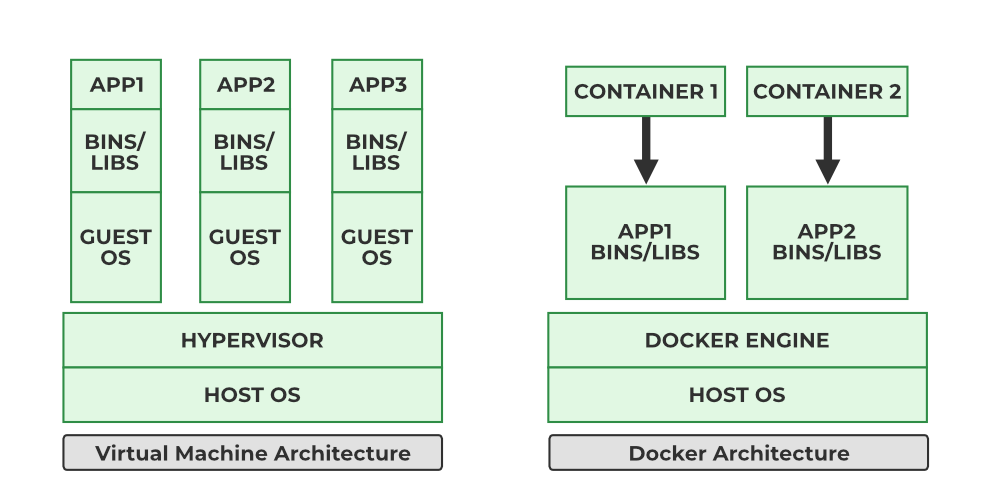
\includegraphics[width=0.9\textwidth,height=0.45\textheight,keepaspectratio]{assets/gambar/landasan-teori/vm_vs_docker.png}%
  }{%
    \framebox[\textwidth][c]{\rule{0pt}{3.5cm}\parbox{0.82\textwidth}{\centering \textbf{[Placeholder Diagram: Perbandingan Arsitektur \textit{Virtual Machine} dan Kontainer Docker]}\\\textit{Menampilkan tumpukan Hypervisor + Guest OS vs Docker Engine berbagi Host OS Kernel. (Menunggu berkas gambar)}}}}
  \caption{Perbandingan Arsitektur \textit{Virtual Machine} Tradisional dan Kontainerisasi Docker}
  \label{fig:teori_docker_vm}
\end{figure}

Berdasarkan Gambar~\ref{fig:teori_docker_vm}, hilangnya lapisan \textit{Guest OS} pada setiap instans membuat pengembang dapat menjalankan banyak layanan terisolasi pada satu peladen fisik dengan konsistensi perilaku yang identik dari komputer pengembang hingga peladen produksi.

\subsection{Docker Compose}

Untuk mendefinisikan dan menjalankan aplikasi terdistribusi yang terdiri atas banyak kontainer sekaligus, ekosistem Docker menyediakan perkakas orkestrasi deklaratif bernama \textbf{Docker Compose}~\cite{docker_compose}. Melalui satu berkas konfigurasi YAML (\texttt{compose.yaml}), pengembang dapat mengatur topologi layanan, jaringan virtual internal (\textit{bridge network}), penyimpan persisten (\textit{volumes}), variabel lingkungan, serta urutan ketergantungan mulai layanan (\texttt{depends\_on}) dalam satu perintah terpadu. Ketiga proyek kerja praktik memanfaatkan Docker dan Docker Compose untuk menstandarkan lingkungan pengembangan hingga produksi.

%------------------------------------------------------------
\section{SISTEM KONTROL VERSI GIT}
%------------------------------------------------------------

\textbf{Git} adalah sistem kontrol versi terdistribusi (\textit{Distributed Version Control System} / DVCS) yang melacak seluruh riwayat perubahan kode sumber dalam bentuk potret (\textit{snapshots}) sistem berkas dan graf asiklik berarah komit (\textit{DAG of commits})~\cite{chacon2014pro}. Karena bersifat terdistribusi, setiap salinan repositori lokal di komputer pengembang menyimpan riwayat proyek secara utuh, sehingga operasi penelusuran histori, percabangan (\textit{branching}) yang ringan, serta penggabungan kode (\textit{merging} dan \textit{rebasing}) berlangsung cepat tanpa ketergantungan konstan pada peladen pusat~\cite{chacon2014pro}.

Model percabangan untuk pengembangan fitur paralel dan penggabungan kembali ke cabang utama pada Git diilustrasikan pada Gambar~\ref{fig:teori_git}.

\begin{figure}[H]
  \centering
  \IfFileExists{assets/gambar/landasan-teori/git_branching.png}{%
    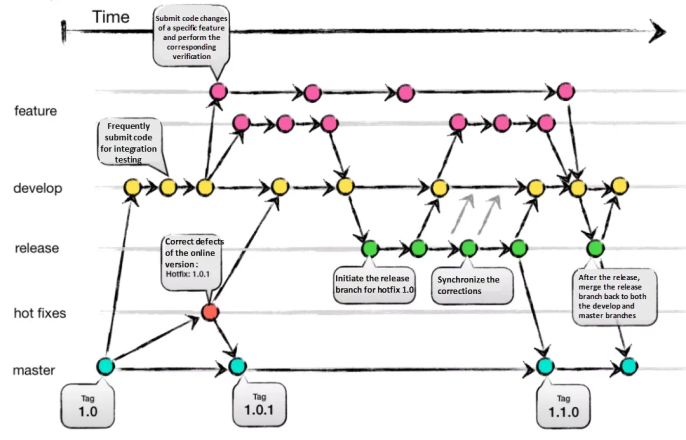
\includegraphics[width=0.9\textwidth,height=0.45\textheight,keepaspectratio]{assets/gambar/landasan-teori/git_branching.png}%
  }{%
    \framebox[\textwidth][c]{\rule{0pt}{3.5cm}\parbox{0.82\textwidth}{\centering \textbf{[Placeholder Diagram: Ilustrasi Model Percabangan dan Penggabungan pada Git]}\\\textit{Menampilkan alur cabang utama main yang bercabang ke feat/* lalu digabung kembali via merge. (Menunggu berkas gambar)}}}}
  \caption{Ilustrasi Model Percabangan (\textit{Branching}) dan Penggabungan (\textit{Merging}) pada Git}
  \label{fig:teori_git}
\end{figure}

Mengacu pada Gambar~\ref{fig:teori_git}, pemisahan pekerjaan fitur atau perbaikan kutu ke cabang tersendiri menjaga stabilitas cabang utama dan memfasilitasi peninjauan kode (\textit{Merge Request}) sebelum integrasi dilakukan.

\subsection{\textit{Conventional Commits}}

Untuk menjaga keterbacaan histori perubahan dan memudahkan audit proyek di \NamaPerusahaan, tim pengembang menerapkan spesifikasi \textbf{\textit{Conventional Commits}}~\cite{conventional_commits}. Standar ini mewajibkan format pesan komit terstruktur berupa \texttt{<type>[optional scope]: <description>}, dengan tipe baku seperti \texttt{feat} untuk penambahan fitur, \texttt{fix} untuk perbaikan kutu, \texttt{docs} untuk dokumentasi, dan \texttt{refactor} untuk pembenahan struktur kode.

%------------------------------------------------------------
\section{CI/CD DAN GITLAB CI/CD}
%------------------------------------------------------------

\textbf{\textit{Continuous Integration} dan \textit{Continuous Delivery/Deployment}} (CI/CD) adalah praktik otomasi rekayasa perangkat lunak yang menjembatani proses pengembangan kode hingga perilisan ke lingkungan operasional~\cite{humble2010continuous}. \textit{Continuous Integration} (CI) menekankan integrasi kode anggota tim secara berkala ke repositori utama yang langsung diverifikasi oleh proses kompilasi, pemeriksaan kualitas statis (\textit{linter}), dan pengujian otomatis guna mendeteksi regresi sedini mungkin. Sementara itu, \textit{Continuous Delivery/Deployment} (CD) mengotomatiskan pengemasan artefak terverifikasi hingga proses perilisan ke lingkungan \textit{staging} maupun produksi secara berulang dan andal~\cite{humble2010continuous}.

Pada proyek kerja praktik, otomasi ini diimplementasikan menggunakan \textbf{GitLab CI/CD} melalui berkas konfigurasi deklaratif \texttt{.gitlab-ci.yml} di dalam masing-masing repositori~\cite{gitlab_cicd}. Alur tahapan otomatis pada \textit{pipeline} GitLab CI/CD diperlihatkan pada Gambar~\ref{fig:teori_cicd}.

\begin{figure}[H]
  \centering
  \IfFileExists{assets/gambar/landasan-teori/gitlab_cicd_pipeline.png}{%
    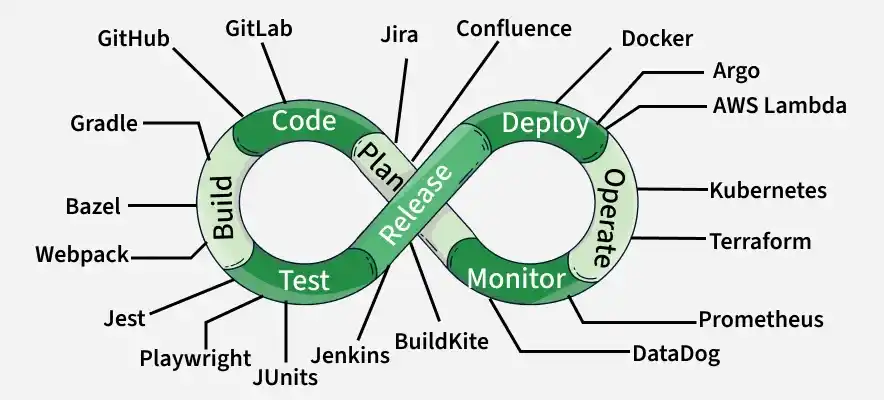
\includegraphics[width=0.92\textwidth,height=0.45\textheight,keepaspectratio]{assets/gambar/landasan-teori/gitlab_cicd_pipeline.png}%
  }{%
    \framebox[\textwidth][c]{\rule{0pt}{3.5cm}\parbox{0.82\textwidth}{\centering \textbf{[Placeholder Diagram: Alur Tahapan Otomatis pada \textit{Pipeline} GitLab CI/CD]}\\\textit{Menampilkan tahapan Git Push $\rightarrow$ Build \& Lint $\rightarrow$ Test $\rightarrow$ Container Registry $\rightarrow$ Deploy. (Menunggu berkas gambar)}}}}
  \caption{Alur Tahapan Otomatis pada \textit{Pipeline} GitLab CI/CD}
  \label{fig:teori_cicd}
\end{figure}

Berdasarkan Gambar~\ref{fig:teori_cicd}, setiap dorongan komit (\textit{push}) atau pengajuan \textit{Merge Request} memicu \textit{GitLab Runner} untuk mengeksekusi tahapan (\textit{stages}) secara berurutan, membangun citra Docker, mengunggah artefak ke \textit{Container Registry}, dan menerapkannya ke peladen target sesuai konfigurasi cabang repositori~\cite{gitlab_cicd}.
